\documentclass[twoside]{book}

% Packages required by doxygen
\usepackage{fixltx2e}
\usepackage{calc}
\usepackage{doxygen}
\usepackage[export]{adjustbox} % also loads graphicx
\usepackage{graphicx}
\usepackage[utf8]{inputenc}
\usepackage{makeidx}
\usepackage{multicol}
\usepackage{multirow}
\PassOptionsToPackage{warn}{textcomp}
\usepackage{textcomp}
\usepackage[nointegrals]{wasysym}
\usepackage[table]{xcolor}

% Font selection
\usepackage[T1]{fontenc}
\usepackage[scaled=.90]{helvet}
\usepackage{courier}
\usepackage{amssymb}
\usepackage{sectsty}
\renewcommand{\familydefault}{\sfdefault}
\allsectionsfont{%
  \fontseries{bc}\selectfont%
  \color{darkgray}%
}
\renewcommand{\DoxyLabelFont}{%
  \fontseries{bc}\selectfont%
  \color{darkgray}%
}
\newcommand{\+}{\discretionary{\mbox{\scriptsize$\hookleftarrow$}}{}{}}

% Page & text layout
\usepackage{geometry}
\geometry{%
  a4paper,%
  top=2.5cm,%
  bottom=2.5cm,%
  left=2.5cm,%
  right=2.5cm%
}
\tolerance=750
\hfuzz=15pt
\hbadness=750
\setlength{\emergencystretch}{15pt}
\setlength{\parindent}{0cm}
\setlength{\parskip}{0.2cm}
\makeatletter
\renewcommand{\paragraph}{%
  \@startsection{paragraph}{4}{0ex}{-1.0ex}{1.0ex}{%
    \normalfont\normalsize\bfseries\SS@parafont%
  }%
}
\renewcommand{\subparagraph}{%
  \@startsection{subparagraph}{5}{0ex}{-1.0ex}{1.0ex}{%
    \normalfont\normalsize\bfseries\SS@subparafont%
  }%
}
\makeatother

% Headers & footers
\usepackage{fancyhdr}
\pagestyle{fancyplain}
\fancyhead[LE]{\fancyplain{}{\bfseries\thepage}}
\fancyhead[CE]{\fancyplain{}{}}
\fancyhead[RE]{\fancyplain{}{\bfseries\leftmark}}
\fancyhead[LO]{\fancyplain{}{\bfseries\rightmark}}
\fancyhead[CO]{\fancyplain{}{}}
\fancyhead[RO]{\fancyplain{}{\bfseries\thepage}}
\fancyfoot[LE]{\fancyplain{}{}}
\fancyfoot[CE]{\fancyplain{}{}}
\fancyfoot[RE]{\fancyplain{}{\bfseries\scriptsize Generated on Sat Jun 6 2015 11\+:37\+:14 for Server Mini\+F\+S by Doxygen }}
\fancyfoot[LO]{\fancyplain{}{\bfseries\scriptsize Generated on Sat Jun 6 2015 11\+:37\+:14 for Server Mini\+F\+S by Doxygen }}
\fancyfoot[CO]{\fancyplain{}{}}
\fancyfoot[RO]{\fancyplain{}{}}
\renewcommand{\footrulewidth}{0.4pt}
\renewcommand{\chaptermark}[1]{%
  \markboth{#1}{}%
}
\renewcommand{\sectionmark}[1]{%
  \markright{\thesection\ #1}%
}

% Indices & bibliography
\usepackage{natbib}
\usepackage[titles]{tocloft}
\setcounter{tocdepth}{3}
\setcounter{secnumdepth}{5}
\makeindex

% Hyperlinks (required, but should be loaded last)
\usepackage{ifpdf}
\ifpdf
  \usepackage[pdftex,pagebackref=true]{hyperref}
\else
  \usepackage[ps2pdf,pagebackref=true]{hyperref}
\fi
\hypersetup{%
  colorlinks=true,%
  linkcolor=blue,%
  citecolor=blue,%
  unicode%
}

% Custom commands
\newcommand{\clearemptydoublepage}{%
  \newpage{\pagestyle{empty}\cleardoublepage}%
}


%===== C O N T E N T S =====

\begin{document}

% Titlepage & ToC
\hypersetup{pageanchor=false,
             bookmarks=true,
             bookmarksnumbered=true,
             pdfencoding=unicode
            }
\pagenumbering{roman}
\begin{titlepage}
\vspace*{7cm}
\begin{center}%
{\Large Server Mini\+F\+S }\\
\vspace*{1cm}
{\large Generated by Doxygen 1.8.9.1}\\
\vspace*{0.5cm}
{\small Sat Jun 6 2015 11:37:14}\\
\end{center}
\end{titlepage}
\clearemptydoublepage
\tableofcontents
\clearemptydoublepage
\pagenumbering{arabic}
\hypersetup{pageanchor=true}

%--- Begin generated contents ---
\chapter{Hierarchical Index}
\section{Class Hierarchy}
This inheritance list is sorted roughly, but not completely, alphabetically\+:\begin{DoxyCompactList}
\item Exception\begin{DoxyCompactList}
\item \contentsline{section}{My\+Base\+Exception}{\pageref{classbloc__device_1_1_my_base_exception}}{}
\begin{DoxyCompactList}
\item \contentsline{section}{Block\+Size\+Error}{\pageref{classbloc__device_1_1_block_size_error}}{}
\item \contentsline{section}{Add\+Entry\+Error}{\pageref{classminixfs_1_1_add_entry_error}}{}
\item \contentsline{section}{Add\+Error}{\pageref{classminixfs_1_1_add_error}}{}
\item \contentsline{section}{Block\+Alloc\+Error}{\pageref{classminixfs_1_1_block_alloc_error}}{}
\item \contentsline{section}{Del\+Entry\+Error}{\pageref{classminixfs_1_1_del_entry_error}}{}
\item \contentsline{section}{Dir\+Full\+Error}{\pageref{classminixfs_1_1_dir_full_error}}{}
\item \contentsline{section}{File\+Name\+Error}{\pageref{classminixfs_1_1_file_name_error}}{}
\item \contentsline{section}{File\+Not\+Found\+Error}{\pageref{classminixfs_1_1_file_not_found_error}}{}
\item \contentsline{section}{Inode\+Error}{\pageref{classminixfs_1_1_inode_error}}{}
\item \contentsline{section}{Outbound\+Error}{\pageref{classminixfs_1_1_outbound_error}}{}
\end{DoxyCompactList}
\item \contentsline{section}{My\+Base\+Exception}{\pageref{classminixfs_1_1_my_base_exception}}{}
\end{DoxyCompactList}
\item object\begin{DoxyCompactList}
\item \contentsline{section}{bloc\+\_\+device}{\pageref{classbloc__device_1_1bloc__device}}{}
\item \contentsline{section}{remote\+\_\+bloc\+\_\+device}{\pageref{classbloc__device_1_1remote__bloc__device}}{}
\item \contentsline{section}{minix\+\_\+inode}{\pageref{classminix__inode_1_1minix__inode}}{}
\item \contentsline{section}{minix\+\_\+superbloc}{\pageref{classminix__superbloc_1_1minix__superbloc}}{}
\item \contentsline{section}{minix\+\_\+file\+\_\+system}{\pageref{classminixfs_1_1minix__file__system}}{}
\end{DoxyCompactList}
\item Test\+Case\begin{DoxyCompactList}
\item \contentsline{section}{Minix\+Tester}{\pageref{classtester2_1_1_minix_tester}}{}
\item \contentsline{section}{Minix\+Tester}{\pageref{classtester_1_1_minix_tester}}{}
\item \contentsline{section}{Minix\+Tester}{\pageref{classtester__server_1_1_minix_tester}}{}
\end{DoxyCompactList}
\end{DoxyCompactList}

\chapter{Data Structure Index}
\section{Data Structures}
Here are the data structures with brief descriptions\+:\begin{DoxyCompactList}
\item\contentsline{section}{\hyperlink{classminixfs_1_1_add_entry_error}{Add\+Entry\+Error} }{\pageref{classminixfs_1_1_add_entry_error}}{}
\item\contentsline{section}{\hyperlink{classminixfs_1_1_add_error}{Add\+Error} }{\pageref{classminixfs_1_1_add_error}}{}
\item\contentsline{section}{\hyperlink{classbloc__device_1_1bloc__device}{bloc\+\_\+device} }{\pageref{classbloc__device_1_1bloc__device}}{}
\item\contentsline{section}{\hyperlink{classminixfs_1_1_block_alloc_error}{Block\+Alloc\+Error} }{\pageref{classminixfs_1_1_block_alloc_error}}{}
\item\contentsline{section}{\hyperlink{classbloc__device_1_1_block_size_error}{Block\+Size\+Error} }{\pageref{classbloc__device_1_1_block_size_error}}{}
\item\contentsline{section}{\hyperlink{classminixfs_1_1_del_entry_error}{Del\+Entry\+Error} }{\pageref{classminixfs_1_1_del_entry_error}}{}
\item\contentsline{section}{\hyperlink{classminixfs_1_1_dir_full_error}{Dir\+Full\+Error} }{\pageref{classminixfs_1_1_dir_full_error}}{}
\item\contentsline{section}{\hyperlink{classminixfs_1_1_file_name_error}{File\+Name\+Error} }{\pageref{classminixfs_1_1_file_name_error}}{}
\item\contentsline{section}{\hyperlink{classminixfs_1_1_file_not_found_error}{File\+Not\+Found\+Error} }{\pageref{classminixfs_1_1_file_not_found_error}}{}
\item\contentsline{section}{\hyperlink{classminixfs_1_1_inode_error}{Inode\+Error} }{\pageref{classminixfs_1_1_inode_error}}{}
\item\contentsline{section}{\hyperlink{classminixfs_1_1minix__file__system}{minix\+\_\+file\+\_\+system} }{\pageref{classminixfs_1_1minix__file__system}}{}
\item\contentsline{section}{\hyperlink{classminix__inode_1_1minix__inode}{minix\+\_\+inode} }{\pageref{classminix__inode_1_1minix__inode}}{}
\item\contentsline{section}{\hyperlink{classminix__superbloc_1_1minix__superbloc}{minix\+\_\+superbloc} }{\pageref{classminix__superbloc_1_1minix__superbloc}}{}
\item\contentsline{section}{\hyperlink{classtester__server_1_1_minix_tester}{Minix\+Tester} }{\pageref{classtester__server_1_1_minix_tester}}{}
\item\contentsline{section}{\hyperlink{classtester_1_1_minix_tester}{Minix\+Tester} }{\pageref{classtester_1_1_minix_tester}}{}
\item\contentsline{section}{\hyperlink{classtester2_1_1_minix_tester}{Minix\+Tester} }{\pageref{classtester2_1_1_minix_tester}}{}
\item\contentsline{section}{\hyperlink{classminixfs_1_1_my_base_exception}{My\+Base\+Exception} }{\pageref{classminixfs_1_1_my_base_exception}}{}
\item\contentsline{section}{\hyperlink{classbloc__device_1_1_my_base_exception}{My\+Base\+Exception} }{\pageref{classbloc__device_1_1_my_base_exception}}{}
\item\contentsline{section}{\hyperlink{classminixfs_1_1_outbound_error}{Outbound\+Error} }{\pageref{classminixfs_1_1_outbound_error}}{}
\item\contentsline{section}{\hyperlink{classbloc__device_1_1remote__bloc__device}{remote\+\_\+bloc\+\_\+device} }{\pageref{classbloc__device_1_1remote__bloc__device}}{}
\end{DoxyCompactList}

\chapter{Data Structure Documentation}
\hypertarget{classminixfs_1_1_add_entry_error}{}\section{Add\+Entry\+Error Class Reference}
\label{classminixfs_1_1_add_entry_error}\index{Add\+Entry\+Error@{Add\+Entry\+Error}}


Inheritance diagram for Add\+Entry\+Error\+:
\nopagebreak
\begin{figure}[H]
\begin{center}
\leavevmode
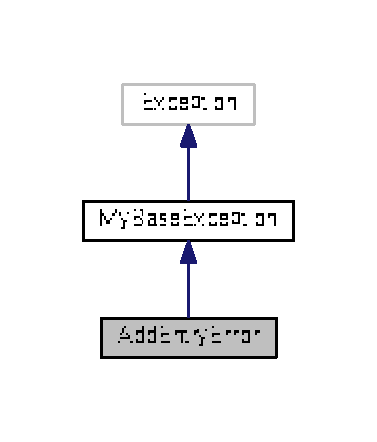
\includegraphics[width=181pt]{classminixfs_1_1_add_entry_error__inherit__graph}
\end{center}
\end{figure}


Collaboration diagram for Add\+Entry\+Error\+:
\nopagebreak
\begin{figure}[H]
\begin{center}
\leavevmode
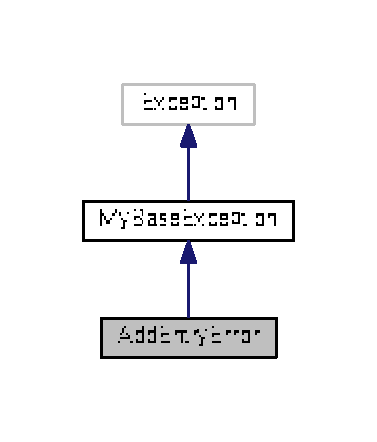
\includegraphics[width=181pt]{classminixfs_1_1_add_entry_error__coll__graph}
\end{center}
\end{figure}
\subsection*{Additional Inherited Members}


The documentation for this class was generated from the following file\+:\begin{DoxyCompactItemize}
\item 
minixfs.\+py\end{DoxyCompactItemize}

\hypertarget{classminixfs_1_1_add_error}{}\section{Add\+Error Class Reference}
\label{classminixfs_1_1_add_error}\index{Add\+Error@{Add\+Error}}


Inheritance diagram for Add\+Error\+:
\nopagebreak
\begin{figure}[H]
\begin{center}
\leavevmode
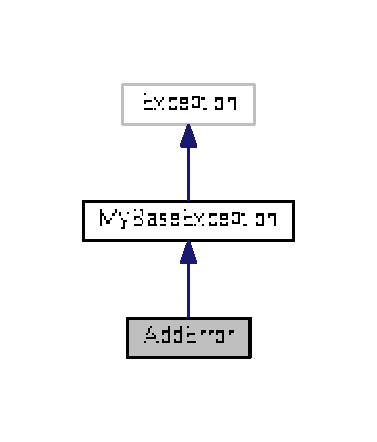
\includegraphics[width=181pt]{classminixfs_1_1_add_error__inherit__graph}
\end{center}
\end{figure}


Collaboration diagram for Add\+Error\+:
\nopagebreak
\begin{figure}[H]
\begin{center}
\leavevmode
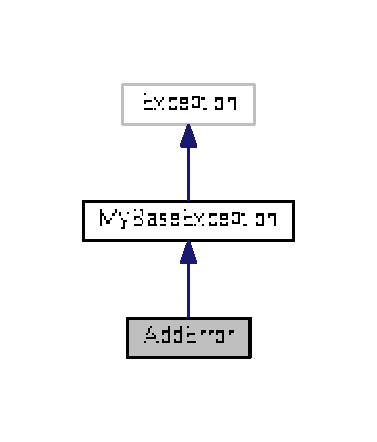
\includegraphics[width=181pt]{classminixfs_1_1_add_error__coll__graph}
\end{center}
\end{figure}
\subsection*{Additional Inherited Members}


The documentation for this class was generated from the following file\+:\begin{DoxyCompactItemize}
\item 
minixfs.\+py\end{DoxyCompactItemize}

\hypertarget{classbloc__device_1_1bloc__device}{}\section{bloc\+\_\+device Class Reference}
\label{classbloc__device_1_1bloc__device}\index{bloc\+\_\+device@{bloc\+\_\+device}}


Inheritance diagram for bloc\+\_\+device\+:
\nopagebreak
\begin{figure}[H]
\begin{center}
\leavevmode
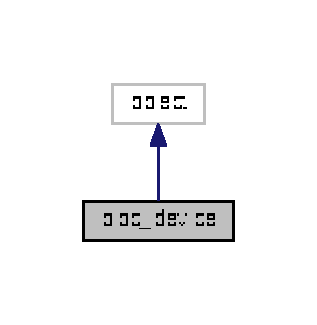
\includegraphics[width=152pt]{classbloc__device_1_1bloc__device__inherit__graph}
\end{center}
\end{figure}


Collaboration diagram for bloc\+\_\+device\+:
\nopagebreak
\begin{figure}[H]
\begin{center}
\leavevmode
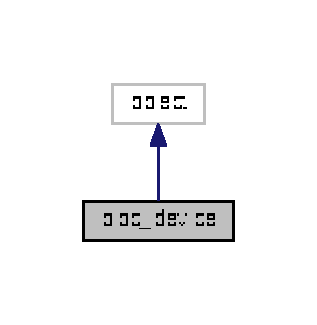
\includegraphics[width=152pt]{classbloc__device_1_1bloc__device__coll__graph}
\end{center}
\end{figure}
\subsection*{Public Member Functions}
\begin{DoxyCompactItemize}
\item 
def \hyperlink{classbloc__device_1_1bloc__device_ac6e95c27b9ae6c994fd74a9314a4fed4}{\+\_\+\+\_\+init\+\_\+\+\_\+} (self, blksize, pathname)
\item 
def \hyperlink{classbloc__device_1_1bloc__device_a41a65d7030dd1006b177d0bc24e1a12b}{\+\_\+\+\_\+del\+\_\+\+\_\+} (self)
\item 
def \hyperlink{classbloc__device_1_1bloc__device_ae8140b2e367967eee2d1e692e1fa09ee}{read\+\_\+bloc}
\item 
def \hyperlink{classbloc__device_1_1bloc__device_a1ebddb0555944a72d7d252d13364b943}{write\+\_\+bloc} (self, bloc\+\_\+num, bloc)
\end{DoxyCompactItemize}
\subsection*{Data Fields}
\begin{DoxyCompactItemize}
\item 
\hypertarget{classbloc__device_1_1bloc__device_a0fe38b9d912af78392a2e7156fbfc6e6}{}{\bfseries blksize}\label{classbloc__device_1_1bloc__device_a0fe38b9d912af78392a2e7156fbfc6e6}

\item 
\hypertarget{classbloc__device_1_1bloc__device_a44f21d5190b5a6df8089f54799628d7e}{}{\bfseries fd}\label{classbloc__device_1_1bloc__device_a44f21d5190b5a6df8089f54799628d7e}

\item 
\hypertarget{classbloc__device_1_1bloc__device_ade010e06fb5903346750389bafe241c2}{}{\bfseries super\+\_\+block}\label{classbloc__device_1_1bloc__device_ade010e06fb5903346750389bafe241c2}

\end{DoxyCompactItemize}


\subsection{Detailed Description}
\begin{DoxyVerb}Class block device \end{DoxyVerb}
 

\subsection{Constructor \& Destructor Documentation}
\hypertarget{classbloc__device_1_1bloc__device_ac6e95c27b9ae6c994fd74a9314a4fed4}{}\index{bloc\+\_\+device\+::bloc\+\_\+device@{bloc\+\_\+device\+::bloc\+\_\+device}!\+\_\+\+\_\+init\+\_\+\+\_\+@{\+\_\+\+\_\+init\+\_\+\+\_\+}}
\index{\+\_\+\+\_\+init\+\_\+\+\_\+@{\+\_\+\+\_\+init\+\_\+\+\_\+}!bloc\+\_\+device\+::bloc\+\_\+device@{bloc\+\_\+device\+::bloc\+\_\+device}}
\subsubsection[{\+\_\+\+\_\+init\+\_\+\+\_\+}]{\setlength{\rightskip}{0pt plus 5cm}def \+\_\+\+\_\+init\+\_\+\+\_\+ (
\begin{DoxyParamCaption}
\item[{}]{self, }
\item[{}]{blksize, }
\item[{}]{pathname}
\end{DoxyParamCaption}
)}\label{classbloc__device_1_1bloc__device_ac6e95c27b9ae6c994fd74a9314a4fed4}
\begin{DoxyVerb}Init a new block device \end{DoxyVerb}
 \hypertarget{classbloc__device_1_1bloc__device_a41a65d7030dd1006b177d0bc24e1a12b}{}\index{bloc\+\_\+device\+::bloc\+\_\+device@{bloc\+\_\+device\+::bloc\+\_\+device}!\+\_\+\+\_\+del\+\_\+\+\_\+@{\+\_\+\+\_\+del\+\_\+\+\_\+}}
\index{\+\_\+\+\_\+del\+\_\+\+\_\+@{\+\_\+\+\_\+del\+\_\+\+\_\+}!bloc\+\_\+device\+::bloc\+\_\+device@{bloc\+\_\+device\+::bloc\+\_\+device}}
\subsubsection[{\+\_\+\+\_\+del\+\_\+\+\_\+}]{\setlength{\rightskip}{0pt plus 5cm}def \+\_\+\+\_\+del\+\_\+\+\_\+ (
\begin{DoxyParamCaption}
\item[{}]{self}
\end{DoxyParamCaption}
)}\label{classbloc__device_1_1bloc__device_a41a65d7030dd1006b177d0bc24e1a12b}
\begin{DoxyVerb}Close properly the block device \end{DoxyVerb}
 

\subsection{Member Function Documentation}
\hypertarget{classbloc__device_1_1bloc__device_ae8140b2e367967eee2d1e692e1fa09ee}{}\index{bloc\+\_\+device\+::bloc\+\_\+device@{bloc\+\_\+device\+::bloc\+\_\+device}!read\+\_\+bloc@{read\+\_\+bloc}}
\index{read\+\_\+bloc@{read\+\_\+bloc}!bloc\+\_\+device\+::bloc\+\_\+device@{bloc\+\_\+device\+::bloc\+\_\+device}}
\subsubsection[{read\+\_\+bloc}]{\setlength{\rightskip}{0pt plus 5cm}def read\+\_\+bloc (
\begin{DoxyParamCaption}
\item[{}]{self, }
\item[{}]{bloc\+\_\+num, }
\item[{}]{numofblk = {\ttfamily 1}}
\end{DoxyParamCaption}
)}\label{classbloc__device_1_1bloc__device_ae8140b2e367967eee2d1e692e1fa09ee}
\begin{DoxyVerb}Read n block from block device
:param bloc_num: block number to be read
:param numofblk: number of block to be read
:return: the buffer
\end{DoxyVerb}
 \hypertarget{classbloc__device_1_1bloc__device_a1ebddb0555944a72d7d252d13364b943}{}\index{bloc\+\_\+device\+::bloc\+\_\+device@{bloc\+\_\+device\+::bloc\+\_\+device}!write\+\_\+bloc@{write\+\_\+bloc}}
\index{write\+\_\+bloc@{write\+\_\+bloc}!bloc\+\_\+device\+::bloc\+\_\+device@{bloc\+\_\+device\+::bloc\+\_\+device}}
\subsubsection[{write\+\_\+bloc}]{\setlength{\rightskip}{0pt plus 5cm}def write\+\_\+bloc (
\begin{DoxyParamCaption}
\item[{}]{self, }
\item[{}]{bloc\+\_\+num, }
\item[{}]{bloc}
\end{DoxyParamCaption}
)}\label{classbloc__device_1_1bloc__device_a1ebddb0555944a72d7d252d13364b943}
\begin{DoxyVerb}Write a block to block device
:param bloc_num: block number to be written
:param bloc: buffer to be written
:return: nb of bytes actually written
\end{DoxyVerb}
 

The documentation for this class was generated from the following file\+:\begin{DoxyCompactItemize}
\item 
bloc\+\_\+device.\+py\end{DoxyCompactItemize}

\hypertarget{classminixfs_1_1_block_alloc_error}{}\section{Block\+Alloc\+Error Class Reference}
\label{classminixfs_1_1_block_alloc_error}\index{Block\+Alloc\+Error@{Block\+Alloc\+Error}}


Inheritance diagram for Block\+Alloc\+Error\+:
\nopagebreak
\begin{figure}[H]
\begin{center}
\leavevmode
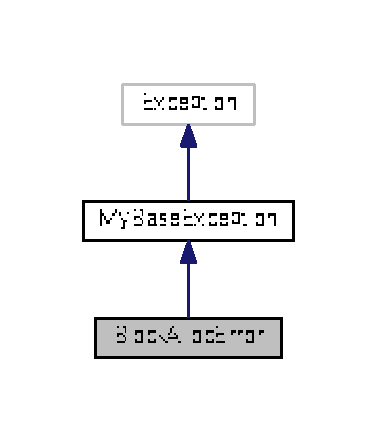
\includegraphics[width=181pt]{classminixfs_1_1_block_alloc_error__inherit__graph}
\end{center}
\end{figure}


Collaboration diagram for Block\+Alloc\+Error\+:
\nopagebreak
\begin{figure}[H]
\begin{center}
\leavevmode
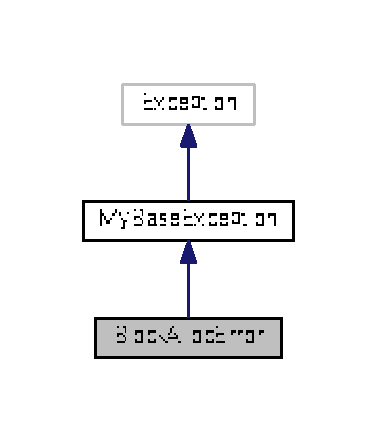
\includegraphics[width=181pt]{classminixfs_1_1_block_alloc_error__coll__graph}
\end{center}
\end{figure}
\subsection*{Additional Inherited Members}


The documentation for this class was generated from the following file\+:\begin{DoxyCompactItemize}
\item 
minixfs.\+py\end{DoxyCompactItemize}

\hypertarget{classbloc__device_1_1_block_size_error}{}\section{Block\+Size\+Error Class Reference}
\label{classbloc__device_1_1_block_size_error}\index{Block\+Size\+Error@{Block\+Size\+Error}}


Inheritance diagram for Block\+Size\+Error\+:
\nopagebreak
\begin{figure}[H]
\begin{center}
\leavevmode
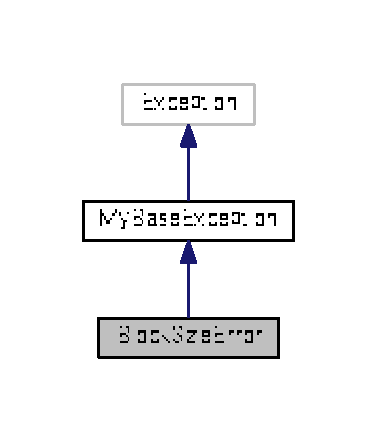
\includegraphics[width=181pt]{classbloc__device_1_1_block_size_error__inherit__graph}
\end{center}
\end{figure}


Collaboration diagram for Block\+Size\+Error\+:
\nopagebreak
\begin{figure}[H]
\begin{center}
\leavevmode
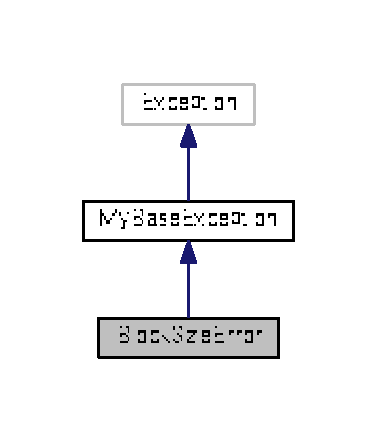
\includegraphics[width=181pt]{classbloc__device_1_1_block_size_error__coll__graph}
\end{center}
\end{figure}
\subsection*{Additional Inherited Members}


The documentation for this class was generated from the following file\+:\begin{DoxyCompactItemize}
\item 
bloc\+\_\+device.\+py\end{DoxyCompactItemize}

\hypertarget{classminixfs_1_1_del_entry_error}{}\section{Del\+Entry\+Error Class Reference}
\label{classminixfs_1_1_del_entry_error}\index{Del\+Entry\+Error@{Del\+Entry\+Error}}


Inheritance diagram for Del\+Entry\+Error\+:
\nopagebreak
\begin{figure}[H]
\begin{center}
\leavevmode
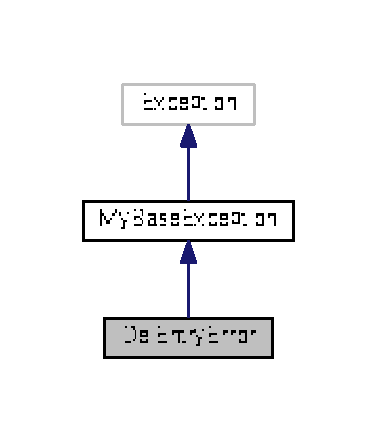
\includegraphics[width=181pt]{classminixfs_1_1_del_entry_error__inherit__graph}
\end{center}
\end{figure}


Collaboration diagram for Del\+Entry\+Error\+:
\nopagebreak
\begin{figure}[H]
\begin{center}
\leavevmode
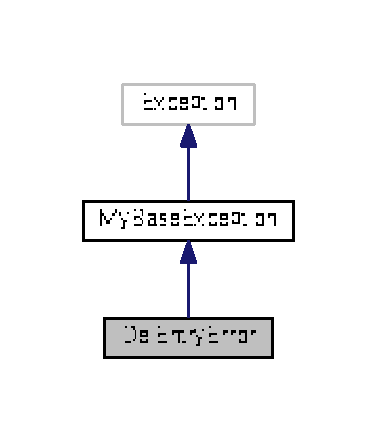
\includegraphics[width=181pt]{classminixfs_1_1_del_entry_error__coll__graph}
\end{center}
\end{figure}
\subsection*{Additional Inherited Members}


The documentation for this class was generated from the following file\+:\begin{DoxyCompactItemize}
\item 
minixfs.\+py\end{DoxyCompactItemize}

\hypertarget{classminixfs_1_1_dir_full_error}{}\section{Dir\+Full\+Error Class Reference}
\label{classminixfs_1_1_dir_full_error}\index{Dir\+Full\+Error@{Dir\+Full\+Error}}


Inheritance diagram for Dir\+Full\+Error\+:
\nopagebreak
\begin{figure}[H]
\begin{center}
\leavevmode
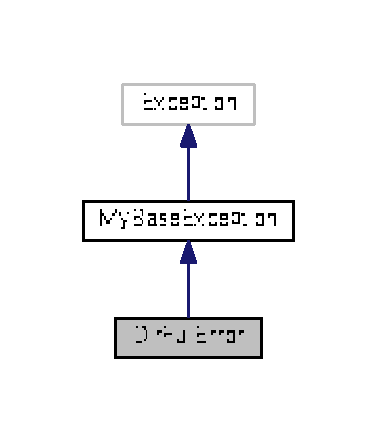
\includegraphics[width=181pt]{classminixfs_1_1_dir_full_error__inherit__graph}
\end{center}
\end{figure}


Collaboration diagram for Dir\+Full\+Error\+:
\nopagebreak
\begin{figure}[H]
\begin{center}
\leavevmode
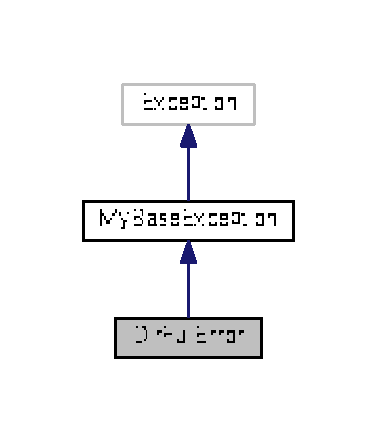
\includegraphics[width=181pt]{classminixfs_1_1_dir_full_error__coll__graph}
\end{center}
\end{figure}
\subsection*{Additional Inherited Members}


The documentation for this class was generated from the following file\+:\begin{DoxyCompactItemize}
\item 
minixfs.\+py\end{DoxyCompactItemize}

\hypertarget{classminixfs_1_1_file_name_error}{}\section{File\+Name\+Error Class Reference}
\label{classminixfs_1_1_file_name_error}\index{File\+Name\+Error@{File\+Name\+Error}}


Inheritance diagram for File\+Name\+Error\+:
\nopagebreak
\begin{figure}[H]
\begin{center}
\leavevmode
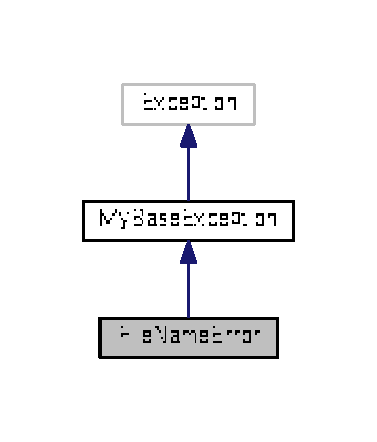
\includegraphics[width=181pt]{classminixfs_1_1_file_name_error__inherit__graph}
\end{center}
\end{figure}


Collaboration diagram for File\+Name\+Error\+:
\nopagebreak
\begin{figure}[H]
\begin{center}
\leavevmode
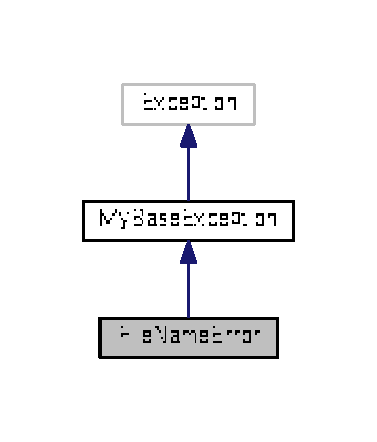
\includegraphics[width=181pt]{classminixfs_1_1_file_name_error__coll__graph}
\end{center}
\end{figure}
\subsection*{Additional Inherited Members}


The documentation for this class was generated from the following file\+:\begin{DoxyCompactItemize}
\item 
minixfs.\+py\end{DoxyCompactItemize}

\hypertarget{classminixfs_1_1_file_not_found_error}{}\section{File\+Not\+Found\+Error Class Reference}
\label{classminixfs_1_1_file_not_found_error}\index{File\+Not\+Found\+Error@{File\+Not\+Found\+Error}}


Inheritance diagram for File\+Not\+Found\+Error\+:
\nopagebreak
\begin{figure}[H]
\begin{center}
\leavevmode
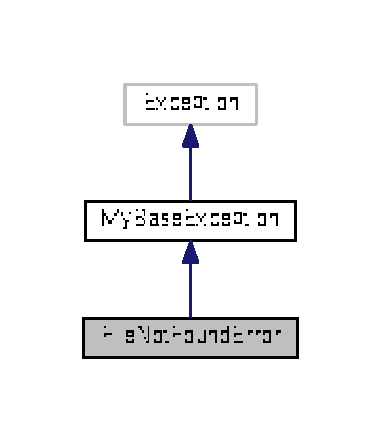
\includegraphics[width=183pt]{classminixfs_1_1_file_not_found_error__inherit__graph}
\end{center}
\end{figure}


Collaboration diagram for File\+Not\+Found\+Error\+:
\nopagebreak
\begin{figure}[H]
\begin{center}
\leavevmode
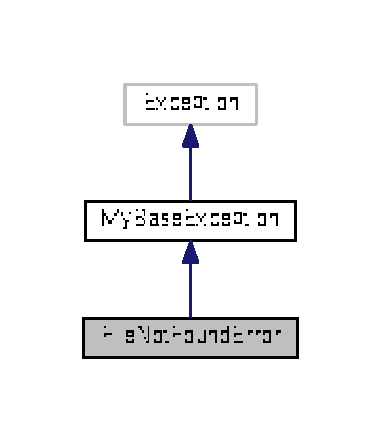
\includegraphics[width=183pt]{classminixfs_1_1_file_not_found_error__coll__graph}
\end{center}
\end{figure}
\subsection*{Additional Inherited Members}


The documentation for this class was generated from the following file\+:\begin{DoxyCompactItemize}
\item 
minixfs.\+py\end{DoxyCompactItemize}

\hypertarget{classminixfs_1_1_inode_error}{}\section{Inode\+Error Class Reference}
\label{classminixfs_1_1_inode_error}\index{Inode\+Error@{Inode\+Error}}


Inheritance diagram for Inode\+Error\+:
\nopagebreak
\begin{figure}[H]
\begin{center}
\leavevmode
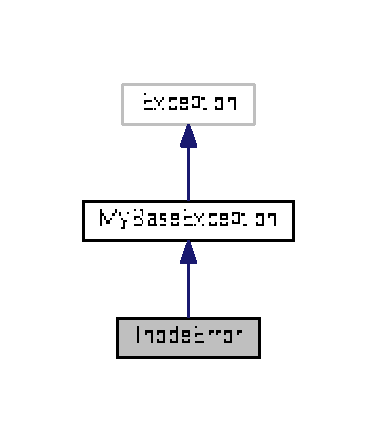
\includegraphics[width=181pt]{classminixfs_1_1_inode_error__inherit__graph}
\end{center}
\end{figure}


Collaboration diagram for Inode\+Error\+:
\nopagebreak
\begin{figure}[H]
\begin{center}
\leavevmode
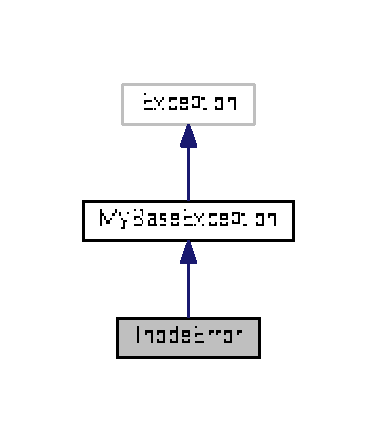
\includegraphics[width=181pt]{classminixfs_1_1_inode_error__coll__graph}
\end{center}
\end{figure}
\subsection*{Additional Inherited Members}


The documentation for this class was generated from the following file\+:\begin{DoxyCompactItemize}
\item 
minixfs.\+py\end{DoxyCompactItemize}

\hypertarget{classminixfs_1_1minix__file__system}{}\section{minix\+\_\+file\+\_\+system Class Reference}
\label{classminixfs_1_1minix__file__system}\index{minix\+\_\+file\+\_\+system@{minix\+\_\+file\+\_\+system}}


Inheritance diagram for minix\+\_\+file\+\_\+system\+:
\nopagebreak
\begin{figure}[H]
\begin{center}
\leavevmode
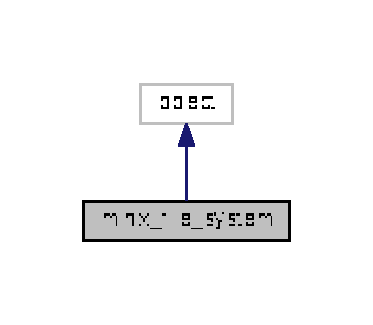
\includegraphics[width=179pt]{classminixfs_1_1minix__file__system__inherit__graph}
\end{center}
\end{figure}


Collaboration diagram for minix\+\_\+file\+\_\+system\+:
\nopagebreak
\begin{figure}[H]
\begin{center}
\leavevmode
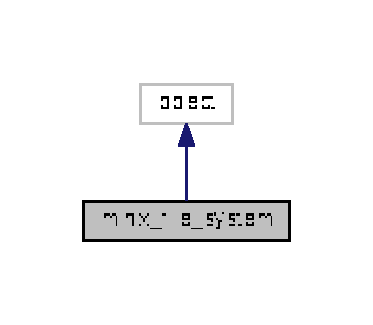
\includegraphics[width=179pt]{classminixfs_1_1minix__file__system__coll__graph}
\end{center}
\end{figure}
\subsection*{Public Member Functions}
\begin{DoxyCompactItemize}
\item 
\hypertarget{classminixfs_1_1minix__file__system_ac775ee34451fdfa742b318538164070e}{}def {\bfseries \+\_\+\+\_\+init\+\_\+\+\_\+}\label{classminixfs_1_1minix__file__system_ac775ee34451fdfa742b318538164070e}

\item 
def \hyperlink{classminixfs_1_1minix__file__system_ac753955974e9b3614eec2d1cf8b93639}{ialloc} (self)
\item 
def \hyperlink{classminixfs_1_1minix__file__system_a55ed46422438bf8eab80de66acd378b1}{ifree} (self, inodnum)
\item 
def \hyperlink{classminixfs_1_1minix__file__system_a51021b42e8af995e5ac74979a7aee885}{balloc} (self)
\item 
def \hyperlink{classminixfs_1_1minix__file__system_a54f50fa051d1d77d753ce8688ed7e6ba}{bfree} (self, blocnum)
\item 
def \hyperlink{classminixfs_1_1minix__file__system_a07b52e5651158cb195a01a5e6234c996}{bmap} (self, inode, blk)
\item 
def \hyperlink{classminixfs_1_1minix__file__system_adf96ecc47840b99f288a32cd06e3abd2}{lookup\+\_\+entry} (self, dinode, name)
\item 
def \hyperlink{classminixfs_1_1minix__file__system_a76146b8729e2a37f75ee55908bee4274}{namei} (self, path)
\item 
def \hyperlink{classminixfs_1_1minix__file__system_a6a0b6aa1991aeb4c025efd78b8ef91b3}{ialloc\+\_\+bloc} (self, ino, blk)
\item 
def \hyperlink{classminixfs_1_1minix__file__system_a166b0076ab0da67e19ff5df78a3d0993}{add\+\_\+entry} (self, dinode, name, new\+\_\+node\+\_\+num)
\item 
def \hyperlink{classminixfs_1_1minix__file__system_af0e1a37032a14afc0f39854b1a9a3b9e}{del\+\_\+entry} (self, dinode, name)
\item 
def \hyperlink{classminixfs_1_1minix__file__system_a000dc714be8532702febb6be755908dc}{close\+\_\+connection} (self)
\item 
def \hyperlink{classminixfs_1_1minix__file__system_ac93c361341836b72c9dce468707c2705}{is\+\_\+dir} (self, inode)
\item 
def \hyperlink{classminixfs_1_1minix__file__system_a293eb36362ad3007d5091e16e2fe6550}{is\+\_\+file} (self, inode)
\item 
def \hyperlink{classminixfs_1_1minix__file__system_a2b4c5bb96e8c76aa6bc4cd4813955e37}{is\+\_\+device} (self, inode)
\item 
def \hyperlink{classminixfs_1_1minix__file__system_aa39b3f3c9b4b0f53db847ec573af0ed7}{is\+\_\+pipe} (self, inode)
\item 
def \hyperlink{classminixfs_1_1minix__file__system_a1ad61c8572bc6ac7095a1fe919f37bff}{is\+\_\+device\+\_\+bloc} (self, inode)
\item 
def \hyperlink{classminixfs_1_1minix__file__system_a8bc62266489b102f6b4355418f7fcc97}{is\+\_\+link} (self, inode)
\item 
def \hyperlink{classminixfs_1_1minix__file__system_ab9c789d57e93f265d894591bc684915d}{update\+\_\+bmap} (self)
\item 
\hypertarget{classminixfs_1_1minix__file__system_a4123373564284dee6575bf8df6bc26b6}{}def {\bfseries write\+\_\+bloc\+\_\+list} (self)\label{classminixfs_1_1minix__file__system_a4123373564284dee6575bf8df6bc26b6}

\end{DoxyCompactItemize}
\subsection*{Data Fields}
\begin{DoxyCompactItemize}
\item 
\hypertarget{classminixfs_1_1minix__file__system_a36c7b5664c44733896398e42189f7c6f}{}{\bfseries disk}\label{classminixfs_1_1minix__file__system_a36c7b5664c44733896398e42189f7c6f}

\item 
\hypertarget{classminixfs_1_1minix__file__system_a1f4f91840a510cd7fc5bcb80c4be2e8d}{}{\bfseries inode\+\_\+map}\label{classminixfs_1_1minix__file__system_a1f4f91840a510cd7fc5bcb80c4be2e8d}

\item 
\hypertarget{classminixfs_1_1minix__file__system_a73bbcc7382e0e5f4e3e39c4d34e823b1}{}{\bfseries zone\+\_\+map}\label{classminixfs_1_1minix__file__system_a73bbcc7382e0e5f4e3e39c4d34e823b1}

\item 
\hypertarget{classminixfs_1_1minix__file__system_ace64866ea69e2b7b947d9ee2b97820a2}{}{\bfseries inodes\+\_\+list}\label{classminixfs_1_1minix__file__system_ace64866ea69e2b7b947d9ee2b97820a2}

\item 
\hypertarget{classminixfs_1_1minix__file__system_ab74e6bf80237ddc4109968cedc58c151}{}{\bfseries name}\label{classminixfs_1_1minix__file__system_ab74e6bf80237ddc4109968cedc58c151}

\item 
\hypertarget{classminixfs_1_1minix__file__system_ac6f54b4e2a370e4eb77474268c5369be}{}{\bfseries inode}\label{classminixfs_1_1minix__file__system_ac6f54b4e2a370e4eb77474268c5369be}

\item 
\hypertarget{classminixfs_1_1minix__file__system_a6858851eee0e05f318897984757b59dc}{}{\bfseries content}\label{classminixfs_1_1minix__file__system_a6858851eee0e05f318897984757b59dc}

\end{DoxyCompactItemize}


\subsection{Detailed Description}
\begin{DoxyVerb}    The main class
\end{DoxyVerb}
 

\subsection{Member Function Documentation}
\hypertarget{classminixfs_1_1minix__file__system_a166b0076ab0da67e19ff5df78a3d0993}{}\index{minixfs\+::minix\+\_\+file\+\_\+system@{minixfs\+::minix\+\_\+file\+\_\+system}!add\+\_\+entry@{add\+\_\+entry}}
\index{add\+\_\+entry@{add\+\_\+entry}!minixfs\+::minix\+\_\+file\+\_\+system@{minixfs\+::minix\+\_\+file\+\_\+system}}
\subsubsection[{add\+\_\+entry}]{\setlength{\rightskip}{0pt plus 5cm}def add\+\_\+entry (
\begin{DoxyParamCaption}
\item[{}]{self, }
\item[{}]{dinode, }
\item[{}]{name, }
\item[{}]{new\+\_\+node\+\_\+num}
\end{DoxyParamCaption}
)}\label{classminixfs_1_1minix__file__system_a166b0076ab0da67e19ff5df78a3d0993}
\begin{DoxyVerb}add a new entry in a dinode (dir)

:param dinode: inode number of the dir
:param name: name of the file to be added
:param new_node_num: inode of the new file
\end{DoxyVerb}
 \hypertarget{classminixfs_1_1minix__file__system_a51021b42e8af995e5ac74979a7aee885}{}\index{minixfs\+::minix\+\_\+file\+\_\+system@{minixfs\+::minix\+\_\+file\+\_\+system}!balloc@{balloc}}
\index{balloc@{balloc}!minixfs\+::minix\+\_\+file\+\_\+system@{minixfs\+::minix\+\_\+file\+\_\+system}}
\subsubsection[{balloc}]{\setlength{\rightskip}{0pt plus 5cm}def balloc (
\begin{DoxyParamCaption}
\item[{}]{self}
\end{DoxyParamCaption}
)}\label{classminixfs_1_1minix__file__system_a51021b42e8af995e5ac74979a7aee885}
\begin{DoxyVerb}return the first free bloc index in the volume.
:return: the first free bloc
\end{DoxyVerb}
 \hypertarget{classminixfs_1_1minix__file__system_a54f50fa051d1d77d753ce8688ed7e6ba}{}\index{minixfs\+::minix\+\_\+file\+\_\+system@{minixfs\+::minix\+\_\+file\+\_\+system}!bfree@{bfree}}
\index{bfree@{bfree}!minixfs\+::minix\+\_\+file\+\_\+system@{minixfs\+::minix\+\_\+file\+\_\+system}}
\subsubsection[{bfree}]{\setlength{\rightskip}{0pt plus 5cm}def bfree (
\begin{DoxyParamCaption}
\item[{}]{self, }
\item[{}]{blocnum}
\end{DoxyParamCaption}
)}\label{classminixfs_1_1minix__file__system_a54f50fa051d1d77d753ce8688ed7e6ba}
\begin{DoxyVerb}toggle a bloc as available for the next balloc()
:param blocnum: blocnum is an index in the zone_map
:return: True if bloc is free
\end{DoxyVerb}
 \hypertarget{classminixfs_1_1minix__file__system_a07b52e5651158cb195a01a5e6234c996}{}\index{minixfs\+::minix\+\_\+file\+\_\+system@{minixfs\+::minix\+\_\+file\+\_\+system}!bmap@{bmap}}
\index{bmap@{bmap}!minixfs\+::minix\+\_\+file\+\_\+system@{minixfs\+::minix\+\_\+file\+\_\+system}}
\subsubsection[{bmap}]{\setlength{\rightskip}{0pt plus 5cm}def bmap (
\begin{DoxyParamCaption}
\item[{}]{self, }
\item[{}]{inode, }
\item[{}]{blk}
\end{DoxyParamCaption}
)}\label{classminixfs_1_1minix__file__system_a07b52e5651158cb195a01a5e6234c996}
\begin{DoxyVerb}Map a block number with his real block number on disk

:param inode: the inode
:param blk: the block number ( 0,.., n-1)
:return: the corresponding block number on disk
\end{DoxyVerb}
 \hypertarget{classminixfs_1_1minix__file__system_a000dc714be8532702febb6be755908dc}{}\index{minixfs\+::minix\+\_\+file\+\_\+system@{minixfs\+::minix\+\_\+file\+\_\+system}!close\+\_\+connection@{close\+\_\+connection}}
\index{close\+\_\+connection@{close\+\_\+connection}!minixfs\+::minix\+\_\+file\+\_\+system@{minixfs\+::minix\+\_\+file\+\_\+system}}
\subsubsection[{close\+\_\+connection}]{\setlength{\rightskip}{0pt plus 5cm}def close\+\_\+connection (
\begin{DoxyParamCaption}
\item[{}]{self}
\end{DoxyParamCaption}
)}\label{classminixfs_1_1minix__file__system_a000dc714be8532702febb6be755908dc}
\begin{DoxyVerb}close connection with remote block server  \end{DoxyVerb}
 \hypertarget{classminixfs_1_1minix__file__system_af0e1a37032a14afc0f39854b1a9a3b9e}{}\index{minixfs\+::minix\+\_\+file\+\_\+system@{minixfs\+::minix\+\_\+file\+\_\+system}!del\+\_\+entry@{del\+\_\+entry}}
\index{del\+\_\+entry@{del\+\_\+entry}!minixfs\+::minix\+\_\+file\+\_\+system@{minixfs\+::minix\+\_\+file\+\_\+system}}
\subsubsection[{del\+\_\+entry}]{\setlength{\rightskip}{0pt plus 5cm}def del\+\_\+entry (
\begin{DoxyParamCaption}
\item[{}]{self, }
\item[{}]{dinode, }
\item[{}]{name}
\end{DoxyParamCaption}
)}\label{classminixfs_1_1minix__file__system_af0e1a37032a14afc0f39854b1a9a3b9e}
\begin{DoxyVerb}delete filename from dir

:param dinode: the directory's file
:param name: filename to remove
\end{DoxyVerb}
 \hypertarget{classminixfs_1_1minix__file__system_ac753955974e9b3614eec2d1cf8b93639}{}\index{minixfs\+::minix\+\_\+file\+\_\+system@{minixfs\+::minix\+\_\+file\+\_\+system}!ialloc@{ialloc}}
\index{ialloc@{ialloc}!minixfs\+::minix\+\_\+file\+\_\+system@{minixfs\+::minix\+\_\+file\+\_\+system}}
\subsubsection[{ialloc}]{\setlength{\rightskip}{0pt plus 5cm}def ialloc (
\begin{DoxyParamCaption}
\item[{}]{self}
\end{DoxyParamCaption}
)}\label{classminixfs_1_1minix__file__system_ac753955974e9b3614eec2d1cf8b93639}
\begin{DoxyVerb}return the first free inode number available
    starting at 0 and upto s.n_inodes-1.
    The bitmap ranges from index 0 to inod_num-1
    Inode 0 is never and is always set.
    according to the inodes bitmap
:return: the first free inode
\end{DoxyVerb}
 \hypertarget{classminixfs_1_1minix__file__system_a6a0b6aa1991aeb4c025efd78b8ef91b3}{}\index{minixfs\+::minix\+\_\+file\+\_\+system@{minixfs\+::minix\+\_\+file\+\_\+system}!ialloc\+\_\+bloc@{ialloc\+\_\+bloc}}
\index{ialloc\+\_\+bloc@{ialloc\+\_\+bloc}!minixfs\+::minix\+\_\+file\+\_\+system@{minixfs\+::minix\+\_\+file\+\_\+system}}
\subsubsection[{ialloc\+\_\+bloc}]{\setlength{\rightskip}{0pt plus 5cm}def ialloc\+\_\+bloc (
\begin{DoxyParamCaption}
\item[{}]{self, }
\item[{}]{ino, }
\item[{}]{blk}
\end{DoxyParamCaption}
)}\label{classminixfs_1_1minix__file__system_a6a0b6aa1991aeb4c025efd78b8ef91b3}
\begin{DoxyVerb}Add a new data block at pos blk and return its real position on disk

:param inode: the inode to add at
:param blk: the block number to add (0,...,n-1)
:return: the block address
\end{DoxyVerb}
 \hypertarget{classminixfs_1_1minix__file__system_a55ed46422438bf8eab80de66acd378b1}{}\index{minixfs\+::minix\+\_\+file\+\_\+system@{minixfs\+::minix\+\_\+file\+\_\+system}!ifree@{ifree}}
\index{ifree@{ifree}!minixfs\+::minix\+\_\+file\+\_\+system@{minixfs\+::minix\+\_\+file\+\_\+system}}
\subsubsection[{ifree}]{\setlength{\rightskip}{0pt plus 5cm}def ifree (
\begin{DoxyParamCaption}
\item[{}]{self, }
\item[{}]{inodnum}
\end{DoxyParamCaption}
)}\label{classminixfs_1_1minix__file__system_a55ed46422438bf8eab80de66acd378b1}
\begin{DoxyVerb}toggle an inode as available for the next ialloc()
:param inodnum:
:return: True if inodnum == False
\end{DoxyVerb}
 \hypertarget{classminixfs_1_1minix__file__system_a2b4c5bb96e8c76aa6bc4cd4813955e37}{}\index{minixfs\+::minix\+\_\+file\+\_\+system@{minixfs\+::minix\+\_\+file\+\_\+system}!is\+\_\+device@{is\+\_\+device}}
\index{is\+\_\+device@{is\+\_\+device}!minixfs\+::minix\+\_\+file\+\_\+system@{minixfs\+::minix\+\_\+file\+\_\+system}}
\subsubsection[{is\+\_\+device}]{\setlength{\rightskip}{0pt plus 5cm}def is\+\_\+device (
\begin{DoxyParamCaption}
\item[{}]{self, }
\item[{}]{inode}
\end{DoxyParamCaption}
)}\label{classminixfs_1_1minix__file__system_a2b4c5bb96e8c76aa6bc4cd4813955e37}
\begin{DoxyVerb}Test if inode is a device
:param inode:
:return: True if inode is a device
\end{DoxyVerb}
 \hypertarget{classminixfs_1_1minix__file__system_a1ad61c8572bc6ac7095a1fe919f37bff}{}\index{minixfs\+::minix\+\_\+file\+\_\+system@{minixfs\+::minix\+\_\+file\+\_\+system}!is\+\_\+device\+\_\+bloc@{is\+\_\+device\+\_\+bloc}}
\index{is\+\_\+device\+\_\+bloc@{is\+\_\+device\+\_\+bloc}!minixfs\+::minix\+\_\+file\+\_\+system@{minixfs\+::minix\+\_\+file\+\_\+system}}
\subsubsection[{is\+\_\+device\+\_\+bloc}]{\setlength{\rightskip}{0pt plus 5cm}def is\+\_\+device\+\_\+bloc (
\begin{DoxyParamCaption}
\item[{}]{self, }
\item[{}]{inode}
\end{DoxyParamCaption}
)}\label{classminixfs_1_1minix__file__system_a1ad61c8572bc6ac7095a1fe919f37bff}
\begin{DoxyVerb}Test if inode is a device bloc
:param inode:
:return: True if inode is a device block
\end{DoxyVerb}
 \hypertarget{classminixfs_1_1minix__file__system_ac93c361341836b72c9dce468707c2705}{}\index{minixfs\+::minix\+\_\+file\+\_\+system@{minixfs\+::minix\+\_\+file\+\_\+system}!is\+\_\+dir@{is\+\_\+dir}}
\index{is\+\_\+dir@{is\+\_\+dir}!minixfs\+::minix\+\_\+file\+\_\+system@{minixfs\+::minix\+\_\+file\+\_\+system}}
\subsubsection[{is\+\_\+dir}]{\setlength{\rightskip}{0pt plus 5cm}def is\+\_\+dir (
\begin{DoxyParamCaption}
\item[{}]{self, }
\item[{}]{inode}
\end{DoxyParamCaption}
)}\label{classminixfs_1_1minix__file__system_ac93c361341836b72c9dce468707c2705}
\begin{DoxyVerb}Test if inode is a dir
:param inode:
:return: True if inode is a dir
\end{DoxyVerb}
 \hypertarget{classminixfs_1_1minix__file__system_a293eb36362ad3007d5091e16e2fe6550}{}\index{minixfs\+::minix\+\_\+file\+\_\+system@{minixfs\+::minix\+\_\+file\+\_\+system}!is\+\_\+file@{is\+\_\+file}}
\index{is\+\_\+file@{is\+\_\+file}!minixfs\+::minix\+\_\+file\+\_\+system@{minixfs\+::minix\+\_\+file\+\_\+system}}
\subsubsection[{is\+\_\+file}]{\setlength{\rightskip}{0pt plus 5cm}def is\+\_\+file (
\begin{DoxyParamCaption}
\item[{}]{self, }
\item[{}]{inode}
\end{DoxyParamCaption}
)}\label{classminixfs_1_1minix__file__system_a293eb36362ad3007d5091e16e2fe6550}
\begin{DoxyVerb}Test if inode is a file
:param inode:
:return: True if inode is a file
\end{DoxyVerb}
 \hypertarget{classminixfs_1_1minix__file__system_a8bc62266489b102f6b4355418f7fcc97}{}\index{minixfs\+::minix\+\_\+file\+\_\+system@{minixfs\+::minix\+\_\+file\+\_\+system}!is\+\_\+link@{is\+\_\+link}}
\index{is\+\_\+link@{is\+\_\+link}!minixfs\+::minix\+\_\+file\+\_\+system@{minixfs\+::minix\+\_\+file\+\_\+system}}
\subsubsection[{is\+\_\+link}]{\setlength{\rightskip}{0pt plus 5cm}def is\+\_\+link (
\begin{DoxyParamCaption}
\item[{}]{self, }
\item[{}]{inode}
\end{DoxyParamCaption}
)}\label{classminixfs_1_1minix__file__system_a8bc62266489b102f6b4355418f7fcc97}
\begin{DoxyVerb}Test if inode is a device link
:param inode:
:return: True if inode is a link
\end{DoxyVerb}
 \hypertarget{classminixfs_1_1minix__file__system_aa39b3f3c9b4b0f53db847ec573af0ed7}{}\index{minixfs\+::minix\+\_\+file\+\_\+system@{minixfs\+::minix\+\_\+file\+\_\+system}!is\+\_\+pipe@{is\+\_\+pipe}}
\index{is\+\_\+pipe@{is\+\_\+pipe}!minixfs\+::minix\+\_\+file\+\_\+system@{minixfs\+::minix\+\_\+file\+\_\+system}}
\subsubsection[{is\+\_\+pipe}]{\setlength{\rightskip}{0pt plus 5cm}def is\+\_\+pipe (
\begin{DoxyParamCaption}
\item[{}]{self, }
\item[{}]{inode}
\end{DoxyParamCaption}
)}\label{classminixfs_1_1minix__file__system_aa39b3f3c9b4b0f53db847ec573af0ed7}
\begin{DoxyVerb}Test if inode is a pipe
:param inode:
:return: True if inode is a pipe
\end{DoxyVerb}
 \hypertarget{classminixfs_1_1minix__file__system_adf96ecc47840b99f288a32cd06e3abd2}{}\index{minixfs\+::minix\+\_\+file\+\_\+system@{minixfs\+::minix\+\_\+file\+\_\+system}!lookup\+\_\+entry@{lookup\+\_\+entry}}
\index{lookup\+\_\+entry@{lookup\+\_\+entry}!minixfs\+::minix\+\_\+file\+\_\+system@{minixfs\+::minix\+\_\+file\+\_\+system}}
\subsubsection[{lookup\+\_\+entry}]{\setlength{\rightskip}{0pt plus 5cm}def lookup\+\_\+entry (
\begin{DoxyParamCaption}
\item[{}]{self, }
\item[{}]{dinode, }
\item[{}]{name}
\end{DoxyParamCaption}
)}\label{classminixfs_1_1minix__file__system_adf96ecc47840b99f288a32cd06e3abd2}
\begin{DoxyVerb}lookup for a name in a directory, and return its inode number,
    given inode directory dinode
:param dinode: directory inode
:param name: dirname to search
:return: directory's inode
\end{DoxyVerb}
 \hypertarget{classminixfs_1_1minix__file__system_a76146b8729e2a37f75ee55908bee4274}{}\index{minixfs\+::minix\+\_\+file\+\_\+system@{minixfs\+::minix\+\_\+file\+\_\+system}!namei@{namei}}
\index{namei@{namei}!minixfs\+::minix\+\_\+file\+\_\+system@{minixfs\+::minix\+\_\+file\+\_\+system}}
\subsubsection[{namei}]{\setlength{\rightskip}{0pt plus 5cm}def namei (
\begin{DoxyParamCaption}
\item[{}]{self, }
\item[{}]{path}
\end{DoxyParamCaption}
)}\label{classminixfs_1_1minix__file__system_a76146b8729e2a37f75ee55908bee4274}
\begin{DoxyVerb}take a path as input and return it's inode number

:param path: path to search
:return: inode of the file
\end{DoxyVerb}
 \hypertarget{classminixfs_1_1minix__file__system_ab9c789d57e93f265d894591bc684915d}{}\index{minixfs\+::minix\+\_\+file\+\_\+system@{minixfs\+::minix\+\_\+file\+\_\+system}!update\+\_\+bmap@{update\+\_\+bmap}}
\index{update\+\_\+bmap@{update\+\_\+bmap}!minixfs\+::minix\+\_\+file\+\_\+system@{minixfs\+::minix\+\_\+file\+\_\+system}}
\subsubsection[{update\+\_\+bmap}]{\setlength{\rightskip}{0pt plus 5cm}def update\+\_\+bmap (
\begin{DoxyParamCaption}
\item[{}]{self}
\end{DoxyParamCaption}
)}\label{classminixfs_1_1minix__file__system_ab9c789d57e93f265d894591bc684915d}
\begin{DoxyVerb}Write bitarray map of data to disk
    cos we need a consistent filesystem
:return: 0
\end{DoxyVerb}
 

The documentation for this class was generated from the following file\+:\begin{DoxyCompactItemize}
\item 
minixfs.\+py\end{DoxyCompactItemize}

\hypertarget{classminix__inode_1_1minix__inode}{}\section{minix\+\_\+inode Class Reference}
\label{classminix__inode_1_1minix__inode}\index{minix\+\_\+inode@{minix\+\_\+inode}}


Inheritance diagram for minix\+\_\+inode\+:
\nopagebreak
\begin{figure}[H]
\begin{center}
\leavevmode
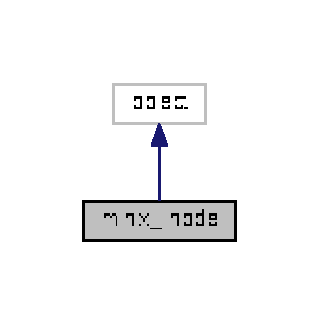
\includegraphics[width=153pt]{classminix__inode_1_1minix__inode__inherit__graph}
\end{center}
\end{figure}


Collaboration diagram for minix\+\_\+inode\+:
\nopagebreak
\begin{figure}[H]
\begin{center}
\leavevmode
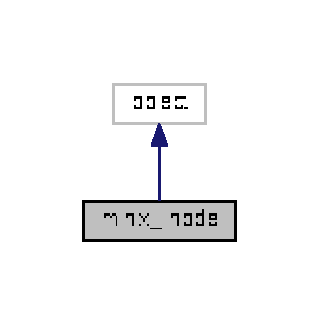
\includegraphics[width=153pt]{classminix__inode_1_1minix__inode__coll__graph}
\end{center}
\end{figure}
\subsection*{Public Member Functions}
\begin{DoxyCompactItemize}
\item 
\hypertarget{classminix__inode_1_1minix__inode_ac775ee34451fdfa742b318538164070e}{}def {\bfseries \+\_\+\+\_\+init\+\_\+\+\_\+}\label{classminix__inode_1_1minix__inode_ac775ee34451fdfa742b318538164070e}

\item 
\hypertarget{classminix__inode_1_1minix__inode_ad794ff077f2f05f228a7109f3670ac40}{}def {\bfseries \+\_\+\+\_\+eq\+\_\+\+\_\+} (self, other)\label{classminix__inode_1_1minix__inode_ad794ff077f2f05f228a7109f3670ac40}

\item 
\hypertarget{classminix__inode_1_1minix__inode_a9a47563093dfc5ba12274b66e368920c}{}def {\bfseries \+\_\+\+\_\+repr\+\_\+\+\_\+} (self)\label{classminix__inode_1_1minix__inode_a9a47563093dfc5ba12274b66e368920c}

\item 
\hypertarget{classminix__inode_1_1minix__inode_aab91ae2e037c39b631a69273c277bfe9}{}def {\bfseries \+\_\+\+\_\+getitem\+\_\+\+\_\+} (self, item)\label{classminix__inode_1_1minix__inode_aab91ae2e037c39b631a69273c277bfe9}

\end{DoxyCompactItemize}
\subsection*{Data Fields}
\begin{DoxyCompactItemize}
\item 
\hypertarget{classminix__inode_1_1minix__inode_a82add66d8c538d243afb8d69b75921e7}{}{\bfseries i\+\_\+ino}\label{classminix__inode_1_1minix__inode_a82add66d8c538d243afb8d69b75921e7}

\item 
\hypertarget{classminix__inode_1_1minix__inode_ade7c443a205890ac8a5952e723ec3565}{}{\bfseries i\+\_\+mode}\label{classminix__inode_1_1minix__inode_ade7c443a205890ac8a5952e723ec3565}

\item 
\hypertarget{classminix__inode_1_1minix__inode_afd70bc57b2985822dea13aeb608bf1a0}{}{\bfseries i\+\_\+uid}\label{classminix__inode_1_1minix__inode_afd70bc57b2985822dea13aeb608bf1a0}

\item 
\hypertarget{classminix__inode_1_1minix__inode_a992f51fcd1d9071641662f9d6f46add2}{}{\bfseries i\+\_\+size}\label{classminix__inode_1_1minix__inode_a992f51fcd1d9071641662f9d6f46add2}

\item 
\hypertarget{classminix__inode_1_1minix__inode_a69a69f7d98750563b632b404005227ca}{}{\bfseries i\+\_\+time}\label{classminix__inode_1_1minix__inode_a69a69f7d98750563b632b404005227ca}

\item 
\hypertarget{classminix__inode_1_1minix__inode_a29fec0e6227c788c16c7cf68d0a739cc}{}{\bfseries i\+\_\+gid}\label{classminix__inode_1_1minix__inode_a29fec0e6227c788c16c7cf68d0a739cc}

\item 
\hypertarget{classminix__inode_1_1minix__inode_a25973b25dacddfa68cf9358f7e29e66e}{}{\bfseries i\+\_\+nlinks}\label{classminix__inode_1_1minix__inode_a25973b25dacddfa68cf9358f7e29e66e}

\item 
\hypertarget{classminix__inode_1_1minix__inode_af8082bd88d3a9e46dd0a4a7de1db9bb2}{}{\bfseries i\+\_\+zone}\label{classminix__inode_1_1minix__inode_af8082bd88d3a9e46dd0a4a7de1db9bb2}

\item 
\hypertarget{classminix__inode_1_1minix__inode_a4d415e5da25984251b4a4efa498dd43c}{}{\bfseries i\+\_\+indir\+\_\+zone}\label{classminix__inode_1_1minix__inode_a4d415e5da25984251b4a4efa498dd43c}

\item 
\hypertarget{classminix__inode_1_1minix__inode_a9fd0ff4ad37e71de47a6a2b82b68a000}{}{\bfseries i\+\_\+dbl\+\_\+indr\+\_\+zone}\label{classminix__inode_1_1minix__inode_a9fd0ff4ad37e71de47a6a2b82b68a000}

\end{DoxyCompactItemize}


\subsection{Detailed Description}
\begin{DoxyVerb}inodes can be initializted from given values or from raw bytes contents coming from the device \end{DoxyVerb}
 

The documentation for this class was generated from the following file\+:\begin{DoxyCompactItemize}
\item 
minix\+\_\+inode.\+py\end{DoxyCompactItemize}

\hypertarget{classminix__superbloc_1_1minix__superbloc}{}\section{minix\+\_\+superbloc Class Reference}
\label{classminix__superbloc_1_1minix__superbloc}\index{minix\+\_\+superbloc@{minix\+\_\+superbloc}}


Inheritance diagram for minix\+\_\+superbloc\+:
\nopagebreak
\begin{figure}[H]
\begin{center}
\leavevmode
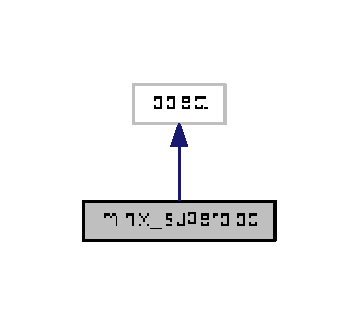
\includegraphics[width=172pt]{classminix__superbloc_1_1minix__superbloc__inherit__graph}
\end{center}
\end{figure}


Collaboration diagram for minix\+\_\+superbloc\+:
\nopagebreak
\begin{figure}[H]
\begin{center}
\leavevmode
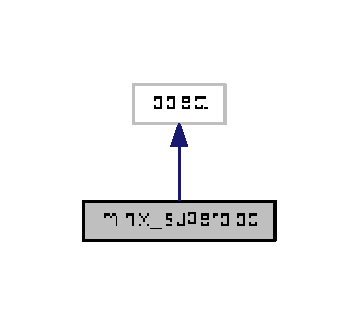
\includegraphics[width=172pt]{classminix__superbloc_1_1minix__superbloc__coll__graph}
\end{center}
\end{figure}
\subsection*{Public Member Functions}
\begin{DoxyCompactItemize}
\item 
def \hyperlink{classminix__superbloc_1_1minix__superbloc_a4c190e7d1ee87ddf6a8b4540bda401bb}{\+\_\+\+\_\+init\+\_\+\+\_\+} (self, blk\+\_\+device)
\end{DoxyCompactItemize}
\subsection*{Data Fields}
\begin{DoxyCompactItemize}
\item 
\hypertarget{classminix__superbloc_1_1minix__superbloc_ace060a1ca09ec7d7b7ad4476f9e46b20}{}{\bfseries s\+\_\+state}\label{classminix__superbloc_1_1minix__superbloc_ace060a1ca09ec7d7b7ad4476f9e46b20}

\end{DoxyCompactItemize}


\subsection{Constructor \& Destructor Documentation}
\hypertarget{classminix__superbloc_1_1minix__superbloc_a4c190e7d1ee87ddf6a8b4540bda401bb}{}\index{minix\+\_\+superbloc\+::minix\+\_\+superbloc@{minix\+\_\+superbloc\+::minix\+\_\+superbloc}!\+\_\+\+\_\+init\+\_\+\+\_\+@{\+\_\+\+\_\+init\+\_\+\+\_\+}}
\index{\+\_\+\+\_\+init\+\_\+\+\_\+@{\+\_\+\+\_\+init\+\_\+\+\_\+}!minix\+\_\+superbloc\+::minix\+\_\+superbloc@{minix\+\_\+superbloc\+::minix\+\_\+superbloc}}
\subsubsection[{\+\_\+\+\_\+init\+\_\+\+\_\+}]{\setlength{\rightskip}{0pt plus 5cm}def \+\_\+\+\_\+init\+\_\+\+\_\+ (
\begin{DoxyParamCaption}
\item[{}]{self, }
\item[{}]{blk\+\_\+device}
\end{DoxyParamCaption}
)}\label{classminix__superbloc_1_1minix__superbloc_a4c190e7d1ee87ddf6a8b4540bda401bb}
\begin{DoxyVerb}Init the super block
:param blk_device: the block device
\end{DoxyVerb}
 

The documentation for this class was generated from the following file\+:\begin{DoxyCompactItemize}
\item 
minix\+\_\+superbloc.\+py\end{DoxyCompactItemize}

\hypertarget{classtester__server_1_1_minix_tester}{}\section{Minix\+Tester Class Reference}
\label{classtester__server_1_1_minix_tester}\index{Minix\+Tester@{Minix\+Tester}}


Inheritance diagram for Minix\+Tester\+:
\nopagebreak
\begin{figure}[H]
\begin{center}
\leavevmode
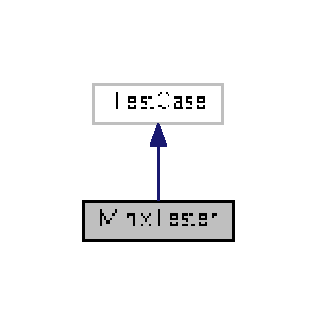
\includegraphics[width=152pt]{classtester__server_1_1_minix_tester__inherit__graph}
\end{center}
\end{figure}


Collaboration diagram for Minix\+Tester\+:
\nopagebreak
\begin{figure}[H]
\begin{center}
\leavevmode
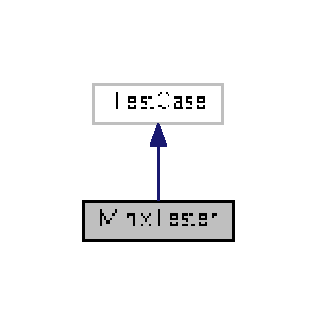
\includegraphics[width=152pt]{classtester__server_1_1_minix_tester__coll__graph}
\end{center}
\end{figure}
\subsection*{Public Member Functions}
\begin{DoxyCompactItemize}
\item 
\hypertarget{classtester__server_1_1_minix_tester_ace7a146509eac31cfc0fc80de9403b08}{}def {\bfseries test\+\_\+1\+\_\+bloc\+\_\+device\+\_\+read\+\_\+bloc} (self)\label{classtester__server_1_1_minix_tester_ace7a146509eac31cfc0fc80de9403b08}

\item 
\hypertarget{classtester__server_1_1_minix_tester_a24a380e585e1ee9c3305c238c83fb736}{}def {\bfseries test\+\_\+2\+\_\+bloc\+\_\+device\+\_\+write\+\_\+bloc} (self)\label{classtester__server_1_1_minix_tester_a24a380e585e1ee9c3305c238c83fb736}

\item 
\hypertarget{classtester__server_1_1_minix_tester_ac80a8db66b10e26951f5b3dbb4ba6177}{}def {\bfseries test\+\_\+3\+\_\+super\+\_\+bloc\+\_\+read\+\_\+super} (self)\label{classtester__server_1_1_minix_tester_ac80a8db66b10e26951f5b3dbb4ba6177}

\item 
\hypertarget{classtester__server_1_1_minix_tester_aea91283fb72bc66c47d112db5b9b0237}{}def {\bfseries test\+\_\+4\+\_\+fs\+\_\+inode\+\_\+and\+\_\+bloc\+\_\+bitmaps} (self)\label{classtester__server_1_1_minix_tester_aea91283fb72bc66c47d112db5b9b0237}

\item 
\hypertarget{classtester__server_1_1_minix_tester_aa84f27bff9f41ed3507faee30ed19958}{}def {\bfseries test\+\_\+5\+\_\+fs\+\_\+inode\+\_\+list} (self)\label{classtester__server_1_1_minix_tester_aa84f27bff9f41ed3507faee30ed19958}

\item 
\hypertarget{classtester__server_1_1_minix_tester_a486e61bd6413ac33f5d2589b1b5eff47}{}def {\bfseries test\+\_\+6\+\_\+fs\+\_\+ialloc\+\_\+ifree} (self)\label{classtester__server_1_1_minix_tester_a486e61bd6413ac33f5d2589b1b5eff47}

\item 
\hypertarget{classtester__server_1_1_minix_tester_a138d86bcce3ab9464a9fae0397358b6d}{}def {\bfseries test\+\_\+7\+\_\+fs\+\_\+balloc\+\_\+bfree} (self)\label{classtester__server_1_1_minix_tester_a138d86bcce3ab9464a9fae0397358b6d}

\item 
\hypertarget{classtester__server_1_1_minix_tester_a9f8509103647b8fec170dc9bd9995d3e}{}def {\bfseries test\+\_\+8\+\_\+fs\+\_\+bmap} (self)\label{classtester__server_1_1_minix_tester_a9f8509103647b8fec170dc9bd9995d3e}

\item 
\hypertarget{classtester__server_1_1_minix_tester_a439662ecb793a5fa39d2a81b82bc3844}{}def {\bfseries test\+\_\+9\+\_\+fs\+\_\+lookup\+\_\+entry} (self)\label{classtester__server_1_1_minix_tester_a439662ecb793a5fa39d2a81b82bc3844}

\item 
\hypertarget{classtester__server_1_1_minix_tester_a2d40ca23d704b6a3dba89feaaa46ef4e}{}def {\bfseries test\+\_\+a\+\_\+fs\+\_\+namei} (self)\label{classtester__server_1_1_minix_tester_a2d40ca23d704b6a3dba89feaaa46ef4e}

\item 
\hypertarget{classtester__server_1_1_minix_tester_aff18c3a4f0015a9a7b9a077ee489a1c4}{}def {\bfseries test\+\_\+b\+\_\+fs\+\_\+ialloc\+\_\+bloc} (self)\label{classtester__server_1_1_minix_tester_aff18c3a4f0015a9a7b9a077ee489a1c4}

\item 
\hypertarget{classtester__server_1_1_minix_tester_a98f3830996534231f31445b8682a5cec}{}def {\bfseries test\+\_\+c\+\_\+fs\+\_\+addentry} (self)\label{classtester__server_1_1_minix_tester_a98f3830996534231f31445b8682a5cec}

\item 
\hypertarget{classtester__server_1_1_minix_tester_a098038e121b2415dbec422f5604bf94c}{}def {\bfseries test\+\_\+d\+\_\+fs\+\_\+delentry} (self)\label{classtester__server_1_1_minix_tester_a098038e121b2415dbec422f5604bf94c}

\end{DoxyCompactItemize}
\subsection*{Data Fields}
\begin{DoxyCompactItemize}
\item 
\hypertarget{classtester__server_1_1_minix_tester_a36c7b5664c44733896398e42189f7c6f}{}{\bfseries disk}\label{classtester__server_1_1_minix_tester_a36c7b5664c44733896398e42189f7c6f}

\item 
\hypertarget{classtester__server_1_1_minix_tester_afbd779c08c2307f759986f8ade741268}{}{\bfseries minixfs}\label{classtester__server_1_1_minix_tester_afbd779c08c2307f759986f8ade741268}

\end{DoxyCompactItemize}


The documentation for this class was generated from the following file\+:\begin{DoxyCompactItemize}
\item 
tester\+\_\+server.\+py\end{DoxyCompactItemize}

\hypertarget{classtester_1_1_minix_tester}{}\section{Minix\+Tester Class Reference}
\label{classtester_1_1_minix_tester}\index{Minix\+Tester@{Minix\+Tester}}


Inheritance diagram for Minix\+Tester\+:
\nopagebreak
\begin{figure}[H]
\begin{center}
\leavevmode
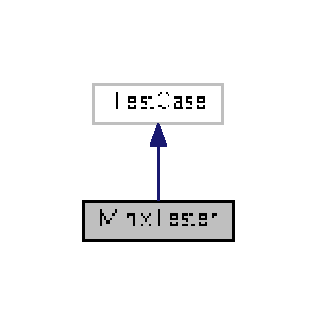
\includegraphics[width=152pt]{classtester_1_1_minix_tester__inherit__graph}
\end{center}
\end{figure}


Collaboration diagram for Minix\+Tester\+:
\nopagebreak
\begin{figure}[H]
\begin{center}
\leavevmode
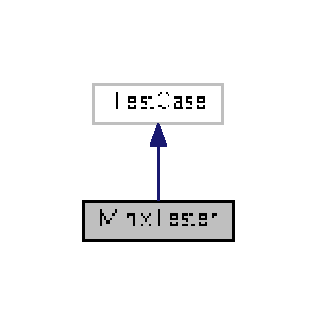
\includegraphics[width=152pt]{classtester_1_1_minix_tester__coll__graph}
\end{center}
\end{figure}
\subsection*{Public Member Functions}
\begin{DoxyCompactItemize}
\item 
\hypertarget{classtester_1_1_minix_tester_ace7a146509eac31cfc0fc80de9403b08}{}def {\bfseries test\+\_\+1\+\_\+bloc\+\_\+device\+\_\+read\+\_\+bloc} (self)\label{classtester_1_1_minix_tester_ace7a146509eac31cfc0fc80de9403b08}

\item 
\hypertarget{classtester_1_1_minix_tester_a24a380e585e1ee9c3305c238c83fb736}{}def {\bfseries test\+\_\+2\+\_\+bloc\+\_\+device\+\_\+write\+\_\+bloc} (self)\label{classtester_1_1_minix_tester_a24a380e585e1ee9c3305c238c83fb736}

\item 
\hypertarget{classtester_1_1_minix_tester_ac80a8db66b10e26951f5b3dbb4ba6177}{}def {\bfseries test\+\_\+3\+\_\+super\+\_\+bloc\+\_\+read\+\_\+super} (self)\label{classtester_1_1_minix_tester_ac80a8db66b10e26951f5b3dbb4ba6177}

\item 
\hypertarget{classtester_1_1_minix_tester_aea91283fb72bc66c47d112db5b9b0237}{}def {\bfseries test\+\_\+4\+\_\+fs\+\_\+inode\+\_\+and\+\_\+bloc\+\_\+bitmaps} (self)\label{classtester_1_1_minix_tester_aea91283fb72bc66c47d112db5b9b0237}

\item 
\hypertarget{classtester_1_1_minix_tester_aa84f27bff9f41ed3507faee30ed19958}{}def {\bfseries test\+\_\+5\+\_\+fs\+\_\+inode\+\_\+list} (self)\label{classtester_1_1_minix_tester_aa84f27bff9f41ed3507faee30ed19958}

\item 
\hypertarget{classtester_1_1_minix_tester_a486e61bd6413ac33f5d2589b1b5eff47}{}def {\bfseries test\+\_\+6\+\_\+fs\+\_\+ialloc\+\_\+ifree} (self)\label{classtester_1_1_minix_tester_a486e61bd6413ac33f5d2589b1b5eff47}

\item 
\hypertarget{classtester_1_1_minix_tester_a138d86bcce3ab9464a9fae0397358b6d}{}def {\bfseries test\+\_\+7\+\_\+fs\+\_\+balloc\+\_\+bfree} (self)\label{classtester_1_1_minix_tester_a138d86bcce3ab9464a9fae0397358b6d}

\item 
\hypertarget{classtester_1_1_minix_tester_a9f8509103647b8fec170dc9bd9995d3e}{}def {\bfseries test\+\_\+8\+\_\+fs\+\_\+bmap} (self)\label{classtester_1_1_minix_tester_a9f8509103647b8fec170dc9bd9995d3e}

\item 
\hypertarget{classtester_1_1_minix_tester_a439662ecb793a5fa39d2a81b82bc3844}{}def {\bfseries test\+\_\+9\+\_\+fs\+\_\+lookup\+\_\+entry} (self)\label{classtester_1_1_minix_tester_a439662ecb793a5fa39d2a81b82bc3844}

\item 
\hypertarget{classtester_1_1_minix_tester_a2d40ca23d704b6a3dba89feaaa46ef4e}{}def {\bfseries test\+\_\+a\+\_\+fs\+\_\+namei} (self)\label{classtester_1_1_minix_tester_a2d40ca23d704b6a3dba89feaaa46ef4e}

\item 
\hypertarget{classtester_1_1_minix_tester_aff18c3a4f0015a9a7b9a077ee489a1c4}{}def {\bfseries test\+\_\+b\+\_\+fs\+\_\+ialloc\+\_\+bloc} (self)\label{classtester_1_1_minix_tester_aff18c3a4f0015a9a7b9a077ee489a1c4}

\item 
\hypertarget{classtester_1_1_minix_tester_a98f3830996534231f31445b8682a5cec}{}def {\bfseries test\+\_\+c\+\_\+fs\+\_\+addentry} (self)\label{classtester_1_1_minix_tester_a98f3830996534231f31445b8682a5cec}

\item 
\hypertarget{classtester_1_1_minix_tester_a098038e121b2415dbec422f5604bf94c}{}def {\bfseries test\+\_\+d\+\_\+fs\+\_\+delentry} (self)\label{classtester_1_1_minix_tester_a098038e121b2415dbec422f5604bf94c}

\item 
\hypertarget{classtester_1_1_minix_tester_a97a872c974641d654f3c414bf46678e8}{}def {\bfseries test\+\_\+e\+\_\+cleanup} (self)\label{classtester_1_1_minix_tester_a97a872c974641d654f3c414bf46678e8}

\end{DoxyCompactItemize}
\subsection*{Data Fields}
\begin{DoxyCompactItemize}
\item 
\hypertarget{classtester_1_1_minix_tester_a36c7b5664c44733896398e42189f7c6f}{}{\bfseries disk}\label{classtester_1_1_minix_tester_a36c7b5664c44733896398e42189f7c6f}

\item 
\hypertarget{classtester_1_1_minix_tester_afbd779c08c2307f759986f8ade741268}{}{\bfseries minixfs}\label{classtester_1_1_minix_tester_afbd779c08c2307f759986f8ade741268}

\end{DoxyCompactItemize}


The documentation for this class was generated from the following file\+:\begin{DoxyCompactItemize}
\item 
tester.\+py\end{DoxyCompactItemize}

\hypertarget{classtester2_1_1_minix_tester}{}\section{Minix\+Tester Class Reference}
\label{classtester2_1_1_minix_tester}\index{Minix\+Tester@{Minix\+Tester}}


Inheritance diagram for Minix\+Tester\+:
\nopagebreak
\begin{figure}[H]
\begin{center}
\leavevmode
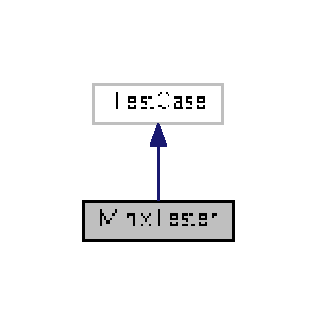
\includegraphics[width=152pt]{classtester2_1_1_minix_tester__inherit__graph}
\end{center}
\end{figure}


Collaboration diagram for Minix\+Tester\+:
\nopagebreak
\begin{figure}[H]
\begin{center}
\leavevmode
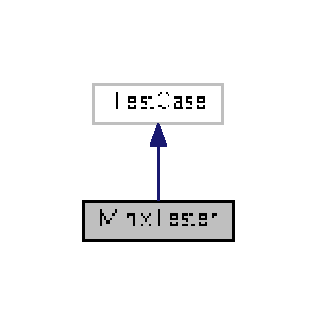
\includegraphics[width=152pt]{classtester2_1_1_minix_tester__coll__graph}
\end{center}
\end{figure}
\subsection*{Public Member Functions}
\begin{DoxyCompactItemize}
\item 
\hypertarget{classtester2_1_1_minix_tester_ace7a146509eac31cfc0fc80de9403b08}{}def {\bfseries test\+\_\+1\+\_\+bloc\+\_\+device\+\_\+read\+\_\+bloc} (self)\label{classtester2_1_1_minix_tester_ace7a146509eac31cfc0fc80de9403b08}

\item 
\hypertarget{classtester2_1_1_minix_tester_a24a380e585e1ee9c3305c238c83fb736}{}def {\bfseries test\+\_\+2\+\_\+bloc\+\_\+device\+\_\+write\+\_\+bloc} (self)\label{classtester2_1_1_minix_tester_a24a380e585e1ee9c3305c238c83fb736}

\item 
\hypertarget{classtester2_1_1_minix_tester_ac80a8db66b10e26951f5b3dbb4ba6177}{}def {\bfseries test\+\_\+3\+\_\+super\+\_\+bloc\+\_\+read\+\_\+super} (self)\label{classtester2_1_1_minix_tester_ac80a8db66b10e26951f5b3dbb4ba6177}

\item 
\hypertarget{classtester2_1_1_minix_tester_aea91283fb72bc66c47d112db5b9b0237}{}def {\bfseries test\+\_\+4\+\_\+fs\+\_\+inode\+\_\+and\+\_\+bloc\+\_\+bitmaps} (self)\label{classtester2_1_1_minix_tester_aea91283fb72bc66c47d112db5b9b0237}

\item 
\hypertarget{classtester2_1_1_minix_tester_a486e61bd6413ac33f5d2589b1b5eff47}{}def {\bfseries test\+\_\+6\+\_\+fs\+\_\+ialloc\+\_\+ifree} (self)\label{classtester2_1_1_minix_tester_a486e61bd6413ac33f5d2589b1b5eff47}

\item 
\hypertarget{classtester2_1_1_minix_tester_a138d86bcce3ab9464a9fae0397358b6d}{}def {\bfseries test\+\_\+7\+\_\+fs\+\_\+balloc\+\_\+bfree} (self)\label{classtester2_1_1_minix_tester_a138d86bcce3ab9464a9fae0397358b6d}

\item 
\hypertarget{classtester2_1_1_minix_tester_a9f8509103647b8fec170dc9bd9995d3e}{}def {\bfseries test\+\_\+8\+\_\+fs\+\_\+bmap} (self)\label{classtester2_1_1_minix_tester_a9f8509103647b8fec170dc9bd9995d3e}

\item 
\hypertarget{classtester2_1_1_minix_tester_a439662ecb793a5fa39d2a81b82bc3844}{}def {\bfseries test\+\_\+9\+\_\+fs\+\_\+lookup\+\_\+entry} (self)\label{classtester2_1_1_minix_tester_a439662ecb793a5fa39d2a81b82bc3844}

\item 
\hypertarget{classtester2_1_1_minix_tester_a2d40ca23d704b6a3dba89feaaa46ef4e}{}def {\bfseries test\+\_\+a\+\_\+fs\+\_\+namei} (self)\label{classtester2_1_1_minix_tester_a2d40ca23d704b6a3dba89feaaa46ef4e}

\item 
\hypertarget{classtester2_1_1_minix_tester_aff18c3a4f0015a9a7b9a077ee489a1c4}{}def {\bfseries test\+\_\+b\+\_\+fs\+\_\+ialloc\+\_\+bloc} (self)\label{classtester2_1_1_minix_tester_aff18c3a4f0015a9a7b9a077ee489a1c4}

\item 
\hypertarget{classtester2_1_1_minix_tester_a98f3830996534231f31445b8682a5cec}{}def {\bfseries test\+\_\+c\+\_\+fs\+\_\+addentry} (self)\label{classtester2_1_1_minix_tester_a98f3830996534231f31445b8682a5cec}

\item 
\hypertarget{classtester2_1_1_minix_tester_a098038e121b2415dbec422f5604bf94c}{}def {\bfseries test\+\_\+d\+\_\+fs\+\_\+delentry} (self)\label{classtester2_1_1_minix_tester_a098038e121b2415dbec422f5604bf94c}

\item 
\hypertarget{classtester2_1_1_minix_tester_a97a872c974641d654f3c414bf46678e8}{}def {\bfseries test\+\_\+e\+\_\+cleanup} (self)\label{classtester2_1_1_minix_tester_a97a872c974641d654f3c414bf46678e8}

\end{DoxyCompactItemize}
\subsection*{Data Fields}
\begin{DoxyCompactItemize}
\item 
\hypertarget{classtester2_1_1_minix_tester_a36c7b5664c44733896398e42189f7c6f}{}{\bfseries disk}\label{classtester2_1_1_minix_tester_a36c7b5664c44733896398e42189f7c6f}

\item 
\hypertarget{classtester2_1_1_minix_tester_afbd779c08c2307f759986f8ade741268}{}{\bfseries minixfs}\label{classtester2_1_1_minix_tester_afbd779c08c2307f759986f8ade741268}

\end{DoxyCompactItemize}


The documentation for this class was generated from the following file\+:\begin{DoxyCompactItemize}
\item 
tester2.\+py\end{DoxyCompactItemize}

\hypertarget{classminixfs_1_1_my_base_exception}{}\section{My\+Base\+Exception Class Reference}
\label{classminixfs_1_1_my_base_exception}\index{My\+Base\+Exception@{My\+Base\+Exception}}


Inheritance diagram for My\+Base\+Exception\+:
\nopagebreak
\begin{figure}[H]
\begin{center}
\leavevmode
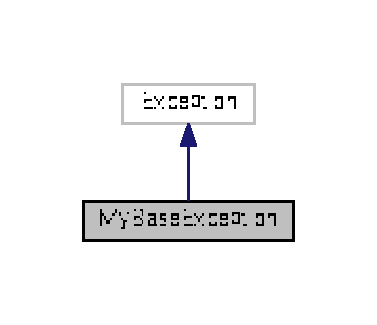
\includegraphics[width=181pt]{classminixfs_1_1_my_base_exception__inherit__graph}
\end{center}
\end{figure}


Collaboration diagram for My\+Base\+Exception\+:
\nopagebreak
\begin{figure}[H]
\begin{center}
\leavevmode
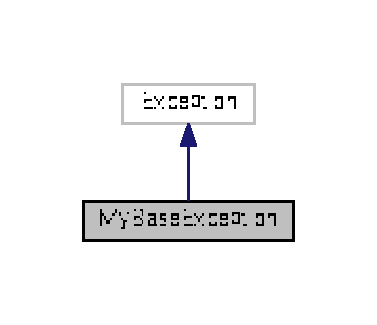
\includegraphics[width=181pt]{classminixfs_1_1_my_base_exception__coll__graph}
\end{center}
\end{figure}
\subsection*{Public Member Functions}
\begin{DoxyCompactItemize}
\item 
\hypertarget{classminixfs_1_1_my_base_exception_a692fa1576e9775a92420b5656e2c00a8}{}def {\bfseries \+\_\+\+\_\+init\+\_\+\+\_\+} (self, message)\label{classminixfs_1_1_my_base_exception_a692fa1576e9775a92420b5656e2c00a8}

\end{DoxyCompactItemize}
\subsection*{Data Fields}
\begin{DoxyCompactItemize}
\item 
\hypertarget{classminixfs_1_1_my_base_exception_ab8140947611504abcb64a4c277effcf5}{}{\bfseries message}\label{classminixfs_1_1_my_base_exception_ab8140947611504abcb64a4c277effcf5}

\end{DoxyCompactItemize}


\subsection{Detailed Description}
\begin{DoxyVerb}Class minixfs exceptions  \end{DoxyVerb}
 

The documentation for this class was generated from the following file\+:\begin{DoxyCompactItemize}
\item 
minixfs.\+py\end{DoxyCompactItemize}

\hypertarget{classbloc__device_1_1_my_base_exception}{}\section{My\+Base\+Exception Class Reference}
\label{classbloc__device_1_1_my_base_exception}\index{My\+Base\+Exception@{My\+Base\+Exception}}


Inheritance diagram for My\+Base\+Exception\+:
\nopagebreak
\begin{figure}[H]
\begin{center}
\leavevmode
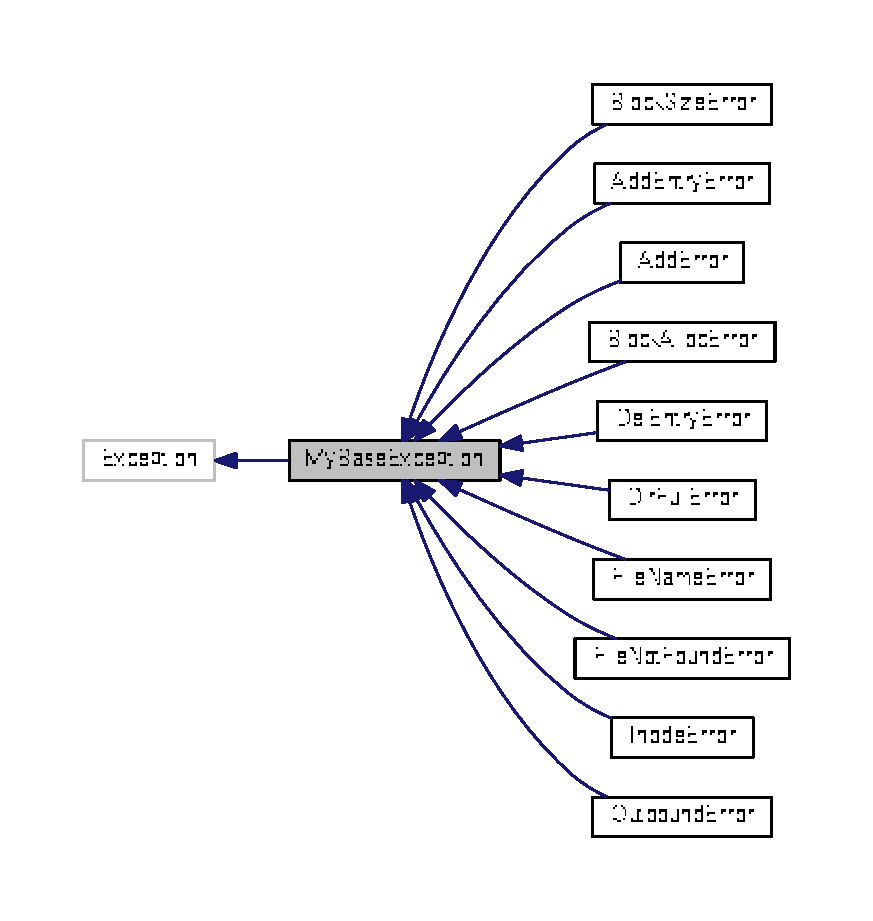
\includegraphics[width=350pt]{classbloc__device_1_1_my_base_exception__inherit__graph}
\end{center}
\end{figure}


Collaboration diagram for My\+Base\+Exception\+:
\nopagebreak
\begin{figure}[H]
\begin{center}
\leavevmode
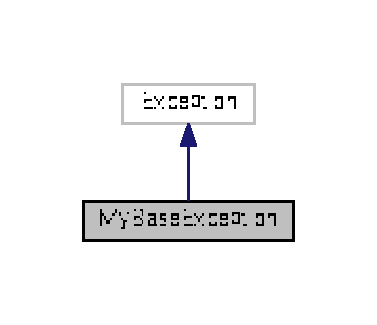
\includegraphics[width=181pt]{classbloc__device_1_1_my_base_exception__coll__graph}
\end{center}
\end{figure}
\subsection*{Public Member Functions}
\begin{DoxyCompactItemize}
\item 
\hypertarget{classbloc__device_1_1_my_base_exception_a692fa1576e9775a92420b5656e2c00a8}{}def {\bfseries \+\_\+\+\_\+init\+\_\+\+\_\+} (self, message)\label{classbloc__device_1_1_my_base_exception_a692fa1576e9775a92420b5656e2c00a8}

\end{DoxyCompactItemize}
\subsection*{Data Fields}
\begin{DoxyCompactItemize}
\item 
\hypertarget{classbloc__device_1_1_my_base_exception_ab8140947611504abcb64a4c277effcf5}{}{\bfseries message}\label{classbloc__device_1_1_my_base_exception_ab8140947611504abcb64a4c277effcf5}

\end{DoxyCompactItemize}


\subsection{Detailed Description}
\begin{DoxyVerb}Class minixfs exceptions  \end{DoxyVerb}
 

The documentation for this class was generated from the following file\+:\begin{DoxyCompactItemize}
\item 
bloc\+\_\+device.\+py\end{DoxyCompactItemize}

\hypertarget{classminixfs_1_1_outbound_error}{}\section{Outbound\+Error Class Reference}
\label{classminixfs_1_1_outbound_error}\index{Outbound\+Error@{Outbound\+Error}}


Inheritance diagram for Outbound\+Error\+:
\nopagebreak
\begin{figure}[H]
\begin{center}
\leavevmode
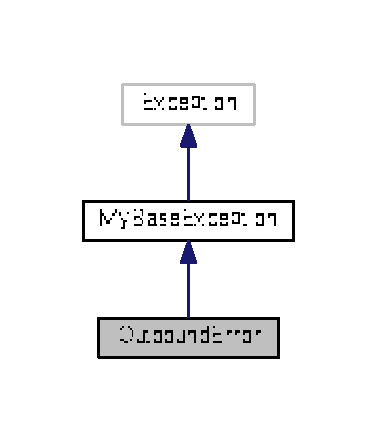
\includegraphics[width=181pt]{classminixfs_1_1_outbound_error__inherit__graph}
\end{center}
\end{figure}


Collaboration diagram for Outbound\+Error\+:
\nopagebreak
\begin{figure}[H]
\begin{center}
\leavevmode
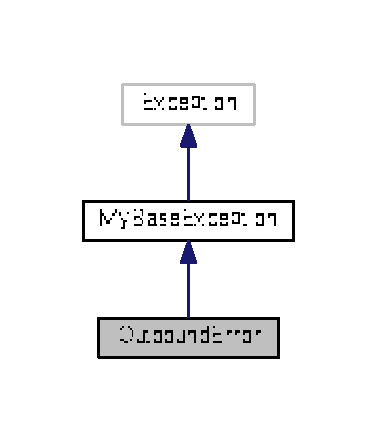
\includegraphics[width=181pt]{classminixfs_1_1_outbound_error__coll__graph}
\end{center}
\end{figure}
\subsection*{Additional Inherited Members}


The documentation for this class was generated from the following file\+:\begin{DoxyCompactItemize}
\item 
minixfs.\+py\end{DoxyCompactItemize}

\hypertarget{classbloc__device_1_1remote__bloc__device}{}\section{remote\+\_\+bloc\+\_\+device Class Reference}
\label{classbloc__device_1_1remote__bloc__device}\index{remote\+\_\+bloc\+\_\+device@{remote\+\_\+bloc\+\_\+device}}


Inheritance diagram for remote\+\_\+bloc\+\_\+device\+:
\nopagebreak
\begin{figure}[H]
\begin{center}
\leavevmode
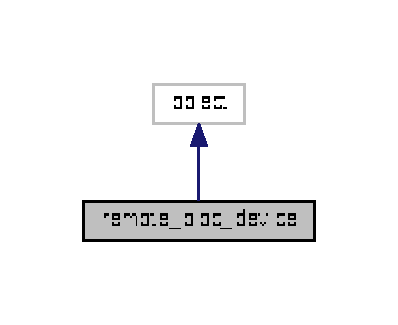
\includegraphics[width=191pt]{classbloc__device_1_1remote__bloc__device__inherit__graph}
\end{center}
\end{figure}


Collaboration diagram for remote\+\_\+bloc\+\_\+device\+:
\nopagebreak
\begin{figure}[H]
\begin{center}
\leavevmode
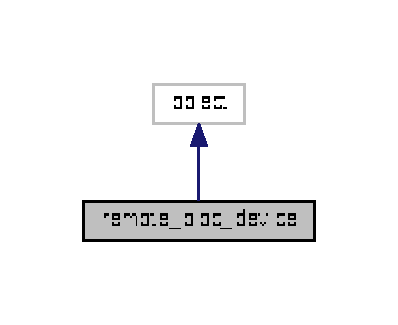
\includegraphics[width=191pt]{classbloc__device_1_1remote__bloc__device__coll__graph}
\end{center}
\end{figure}
\subsection*{Public Member Functions}
\begin{DoxyCompactItemize}
\item 
\hypertarget{classbloc__device_1_1remote__bloc__device_ac775ee34451fdfa742b318538164070e}{}def {\bfseries \+\_\+\+\_\+init\+\_\+\+\_\+}\label{classbloc__device_1_1remote__bloc__device_ac775ee34451fdfa742b318538164070e}

\item 
def \hyperlink{classbloc__device_1_1remote__bloc__device_a41a65d7030dd1006b177d0bc24e1a12b}{\+\_\+\+\_\+del\+\_\+\+\_\+} (self)
\item 
def \hyperlink{classbloc__device_1_1remote__bloc__device_ae8140b2e367967eee2d1e692e1fa09ee}{read\+\_\+bloc}
\item 
def \hyperlink{classbloc__device_1_1remote__bloc__device_a1ebddb0555944a72d7d252d13364b943}{write\+\_\+bloc} (self, bloc\+\_\+num, bloc)
\item 
def \hyperlink{classbloc__device_1_1remote__bloc__device_a000dc714be8532702febb6be755908dc}{close\+\_\+connection} (self)
\end{DoxyCompactItemize}
\subsection*{Data Fields}
\begin{DoxyCompactItemize}
\item 
\hypertarget{classbloc__device_1_1remote__bloc__device_a0fe38b9d912af78392a2e7156fbfc6e6}{}{\bfseries blksize}\label{classbloc__device_1_1remote__bloc__device_a0fe38b9d912af78392a2e7156fbfc6e6}

\item 
\hypertarget{classbloc__device_1_1remote__bloc__device_a796eb6fe3758085a1379a7a873e41fff}{}{\bfseries requests}\label{classbloc__device_1_1remote__bloc__device_a796eb6fe3758085a1379a7a873e41fff}

\item 
\hypertarget{classbloc__device_1_1remote__bloc__device_a7bfddf7ae6ce1b1321289f622d4b117e}{}{\bfseries responses}\label{classbloc__device_1_1remote__bloc__device_a7bfddf7ae6ce1b1321289f622d4b117e}

\item 
\hypertarget{classbloc__device_1_1remote__bloc__device_a44f21d5190b5a6df8089f54799628d7e}{}{\bfseries fd}\label{classbloc__device_1_1remote__bloc__device_a44f21d5190b5a6df8089f54799628d7e}

\item 
\hypertarget{classbloc__device_1_1remote__bloc__device_ade010e06fb5903346750389bafe241c2}{}{\bfseries super\+\_\+block}\label{classbloc__device_1_1remote__bloc__device_ade010e06fb5903346750389bafe241c2}

\end{DoxyCompactItemize}


\subsection{Detailed Description}
\begin{DoxyVerb}Class remote block device

    This class connect to a remote bloc server and
    read/write commands are passed through a
    TCP socket
\end{DoxyVerb}
 

\subsection{Constructor \& Destructor Documentation}
\hypertarget{classbloc__device_1_1remote__bloc__device_a41a65d7030dd1006b177d0bc24e1a12b}{}\index{bloc\+\_\+device\+::remote\+\_\+bloc\+\_\+device@{bloc\+\_\+device\+::remote\+\_\+bloc\+\_\+device}!\+\_\+\+\_\+del\+\_\+\+\_\+@{\+\_\+\+\_\+del\+\_\+\+\_\+}}
\index{\+\_\+\+\_\+del\+\_\+\+\_\+@{\+\_\+\+\_\+del\+\_\+\+\_\+}!bloc\+\_\+device\+::remote\+\_\+bloc\+\_\+device@{bloc\+\_\+device\+::remote\+\_\+bloc\+\_\+device}}
\subsubsection[{\+\_\+\+\_\+del\+\_\+\+\_\+}]{\setlength{\rightskip}{0pt plus 5cm}def \+\_\+\+\_\+del\+\_\+\+\_\+ (
\begin{DoxyParamCaption}
\item[{}]{self}
\end{DoxyParamCaption}
)}\label{classbloc__device_1_1remote__bloc__device_a41a65d7030dd1006b177d0bc24e1a12b}
\begin{DoxyVerb}Cleanly close the socket \end{DoxyVerb}
 

\subsection{Member Function Documentation}
\hypertarget{classbloc__device_1_1remote__bloc__device_a000dc714be8532702febb6be755908dc}{}\index{bloc\+\_\+device\+::remote\+\_\+bloc\+\_\+device@{bloc\+\_\+device\+::remote\+\_\+bloc\+\_\+device}!close\+\_\+connection@{close\+\_\+connection}}
\index{close\+\_\+connection@{close\+\_\+connection}!bloc\+\_\+device\+::remote\+\_\+bloc\+\_\+device@{bloc\+\_\+device\+::remote\+\_\+bloc\+\_\+device}}
\subsubsection[{close\+\_\+connection}]{\setlength{\rightskip}{0pt plus 5cm}def close\+\_\+connection (
\begin{DoxyParamCaption}
\item[{}]{self}
\end{DoxyParamCaption}
)}\label{classbloc__device_1_1remote__bloc__device_a000dc714be8532702febb6be755908dc}
\begin{DoxyVerb}close properly the socket \end{DoxyVerb}
 \hypertarget{classbloc__device_1_1remote__bloc__device_ae8140b2e367967eee2d1e692e1fa09ee}{}\index{bloc\+\_\+device\+::remote\+\_\+bloc\+\_\+device@{bloc\+\_\+device\+::remote\+\_\+bloc\+\_\+device}!read\+\_\+bloc@{read\+\_\+bloc}}
\index{read\+\_\+bloc@{read\+\_\+bloc}!bloc\+\_\+device\+::remote\+\_\+bloc\+\_\+device@{bloc\+\_\+device\+::remote\+\_\+bloc\+\_\+device}}
\subsubsection[{read\+\_\+bloc}]{\setlength{\rightskip}{0pt plus 5cm}def read\+\_\+bloc (
\begin{DoxyParamCaption}
\item[{}]{self, }
\item[{}]{bloc\+\_\+num, }
\item[{}]{numofbloc = {\ttfamily 1}}
\end{DoxyParamCaption}
)}\label{classbloc__device_1_1remote__bloc__device_ae8140b2e367967eee2d1e692e1fa09ee}
\begin{DoxyVerb}Read n block from block device server

:param bloc_num: the bloc number
:param numofbloc: number of block to be read
:return: the response
\end{DoxyVerb}
 \hypertarget{classbloc__device_1_1remote__bloc__device_a1ebddb0555944a72d7d252d13364b943}{}\index{bloc\+\_\+device\+::remote\+\_\+bloc\+\_\+device@{bloc\+\_\+device\+::remote\+\_\+bloc\+\_\+device}!write\+\_\+bloc@{write\+\_\+bloc}}
\index{write\+\_\+bloc@{write\+\_\+bloc}!bloc\+\_\+device\+::remote\+\_\+bloc\+\_\+device@{bloc\+\_\+device\+::remote\+\_\+bloc\+\_\+device}}
\subsubsection[{write\+\_\+bloc}]{\setlength{\rightskip}{0pt plus 5cm}def write\+\_\+bloc (
\begin{DoxyParamCaption}
\item[{}]{self, }
\item[{}]{bloc\+\_\+num, }
\item[{}]{bloc}
\end{DoxyParamCaption}
)}\label{classbloc__device_1_1remote__bloc__device_a1ebddb0555944a72d7d252d13364b943}
\begin{DoxyVerb}Write block from block device server

:param bloc_num: the bloc number
:param bloc: buffer to be written
\end{DoxyVerb}
 

The documentation for this class was generated from the following file\+:\begin{DoxyCompactItemize}
\item 
bloc\+\_\+device.\+py\end{DoxyCompactItemize}

%--- End generated contents ---

% Index
\backmatter
\newpage
\phantomsection
\clearemptydoublepage
\addcontentsline{toc}{chapter}{Index}
\printindex

\end{document}
